%!TEX program = xelatex
\documentclass[12pt,a4paper]{report}

\usepackage{thesis}
\usepackage{lmodern}
\usepackage[numbers,sort&compress]{natbib}
\usepackage[hidelinks]{hyperref}
\usepackage[left=2.5cm,top=2.5cm,right=2.5cm,bottom=2.5cm]{geometry}
\usepackage{nomencl}
\makenomenclature
\renewcommand{\nomname}{ABBREVIATIONS}

\usepackage{amsmath}
\usepackage{ amssymb }
\usepackage{mathtools}
\usepackage{graphicx}
\usepackage{url}
\usepackage{float}
% \usepackage{hyperref}
% \usepackage{paralist}
% \usepackage[parfill]{parskip}
\usepackage{listings}
% \usepackage{xcolor}
\graphicspath{ {images/} }

\usepackage{tocloft}
\usepackage{algorithm}
% \usepackage{algorithmicx}
% \usepackage{algorithmic}
\usepackage[noend]{algpseudocode}

\renewcommand{\cftchapfont}{}
\renewcommand{\cftchappagefont}{}
\renewcommand{\cftdot}{}
\newcommand{\ba}{\mathbf{a}}
\newcommand{\bb}{\mathbf{b}}
\newcommand{\bc}{\mathbf{c}}
\newcommand{\bd}{\mathbf{d}}
\newcommand{\be}{\mathbf{e}}
\newcommand{\bg}{\mathbf{g}}
\newcommand{\bh}{\mathbf{h}}
\newcommand{\bi}{\mathbf{i}}
\newcommand{\bj}{\mathbf{j}}
\newcommand{\bk}{\mathbf{k}}
\newcommand{\bl}{\mathbf{l}}
\newcommand{\bn}{\mathbf{n}}
\newcommand{\bo}{\mathbf{o}}
\newcommand{\bp}{\mathbf{p}}
\newcommand{\bq}{\mathbf{q}}
\newcommand{\br}{\mathbf{r}}
\newcommand{\bs}{\mathbf{s}}
\newcommand{\bt}{\mathbf{t}}
\newcommand{\bu}{\mathbf{u}}
\newcommand{\bv}{\mathbf{v}}
\newcommand{\bw}{\mathbf{w}}
\newcommand{\bx}{\mathbf{x}}
\newcommand{\by}{\mathbf{y}}
\newcommand{\bz}{\mathbf{z}}
\newcommand{\bA}{\mathbf{A}}
\newcommand{\bB}{\mathbf{B}}
\newcommand{\bC}{\mathbf{C}}
\newcommand{\bD}{\mathbf{D}}
\newcommand{\bE}{\mathbf{E}}
\newcommand{\bF}{\mathbf{F}}
\newcommand{\bG}{\mathbf{G}}
\newcommand{\bH}{\mathbf{H}}
\newcommand{\bI}{\mathbf{I}}
\newcommand{\bJ}{\mathbf{J}}
\newcommand{\bK}{\mathbf{K}}
\newcommand{\bL}{\mathbf{L}}
\newcommand{\bM}{\mathbf{M}}
\newcommand{\bN}{\mathbf{N}}
\newcommand{\bO}{\mathbf{O}}
\newcommand{\bP}{\mathbf{P}}
\newcommand{\bQ}{\mathbf{Q}}
\newcommand{\bR}{\mathbf{R}}
\newcommand{\bS}{\mathbf{S}}
\newcommand{\bT}{\mathbf{T}}
\newcommand{\bU}{\mathbf{U}}
\newcommand{\bV}{\mathbf{V}}
\newcommand{\bW}{\mathbf{W}}
\newcommand{\bX}{\mathbf{X}}
\newcommand{\bY}{\mathbf{Y}}
\newcommand{\bZ}{\mathbf{Z}}
\newcommand{\bzero}{\mathbf{0}}
\newcommand{\bone}{\mathbf{1}}
\newcommand{\bdot}{\mathbf{cdot}}
\usepackage{bm}
\newcommand{\bphi}{\bm{\phi}}
\newcommand{\bPhi}{\bm{\Phi}}
\newcommand{\bepsilon}{\bm{\epsilon}}
\newcommand{\bSigma}{\bm{\Sigma}}
\newcommand{\bGamma}{\bm{\Gamma}}
\newcommand{\bbeta}{\bm{\beta}}
\newcommand{\bdelta}{\bm{\delta}}
% GENL MATH
\newcommand{\Real}{\mathbb{R}}
\DeclareMathOperator*{\argmin}{arg\,min}
\DeclareMathOperator*{\argmax}{arg\,max}
\DeclareMathOperator*{\minimize}{minimize}
\DeclareMathOperator*{\maximize}{maximize}
\newcommand{\half}{\frac{1}{2}}
\newcommand{\defeq}{\vcentcolon=}
\newcommand{\given}[1][]{\:#1\vert\:}
\newcommand{\suchthat}{\:\vert\:}
\newcommand{\grad}{\nabla}
\newcommand{\evalat}[1]{\big\rvert_{#1}}

% STATISTICS
\newcommand{\E}{\mathbb{E}}
\newcommand{\Var}{\mathrm{Var}}
\newcommand{\Cov}{\mathrm{Cov}}
\newcommand{\Ea}[1]{\E\left[#1\right]}
\newcommand{\Eb}[2]{\E_{#1}\left[#2\right]}
\newcommand{\Vara}[1]{\Var\left[#1\right]}
\newcommand{\Varb}[2]{\Var_{#1}\left[#2\right]}
\newcommand{\lone}[1]{\norm{#1}_1}

% DELIMITERS
% \newcommand{\lrbrack}[1]{\left[#1\right]}
% \newcommand{\lrbrace}[1]{\left\{#1\right\}}
% \newcommand{\lrparen}[1]{\left(#1\right)}

% NORMS
\DeclarePairedDelimiter{\norm}{\|}{\|}
\DeclarePairedDelimiter{\abs}{|}{|}
\newcommand{\pospart}[1]{\abs{#1}^+}
\DeclarePairedDelimiter{\lrbrack}{[}{]}
\DeclarePairedDelimiter{\lrbrace}{ \{ }{ \} }
\DeclarePairedDelimiter{\lrparen}{(}{)}
\DeclarePairedDelimiter{\lrang}{\langle}{\rangle}
\newcommand{\infnorm}[1]{\norm{#1}_{\infty}}
\newcommand{\normone}[1]{\norm{#1}_1}

% MDP
\newcommand{\cS}{\mathcal{S}}
\newcommand{\cA}{\mathcal{A}}
\newcommand{\adv}{\mathbb{A}}
\newcommand{\rhopi}{\rho_{\pi}}
\newcommand{\Qpi}{\ensuremath{Q^{\pi}}}
\newcommand{\Api}{\ensuremath{A^{\pi}}}
\newcommand{\Vpi}{\ensuremath{V^{\pi}}}
\newcommand{\Qstar}{\ensuremath{Q^{*}}}
\newcommand{\Astar}{\ensuremath{A^{*}}}
\newcommand{\Vstar}{\ensuremath{V^{*}}}

% POLILCY
\newcommand{\piold}{\pi_{old}}
\newcommand{\pinew}{\pi_{new}}
\newcommand{\thold}{\theta_{old}}
\newcommand{\thnew}{\theta_{new}}
\newcommand{\tilth}{\tilde{\theta}}
\newcommand{\pith}{\pi_{\theta}}
\newcommand{\pitilth}{\pi_{\tilth}}
\newcommand{\gradth}{\grad_{\theta}}

% DIVERGENCE
\newcommand{\kl}[2]{D_{KL}(#1 \ \| \ #2)}
\newcommand{\tv}[2]{D_{TV}(#1 \ \| \ #2)}

% MISC
\newcommand{\tdlam}{TD($\lambda$)}
\newcommand{\tdzero}{TD($0$)}
\newcommand{\tdone}{TD($1$)}
\newcommand{\lstdlam}{LSTD($\lambda$)}
\newcommand{\lstdzero}{LSTD($0$)}
\newcommand{\lstdone}{LSTD($1$)}
\newcommand{\brmlam}{BRM($\lambda$)}
\newcommand{\brmzero}{BRM($0$)}
\newcommand{\brmone}{BRM($1$)}
\newcommand{\lspelam}{LSPE($\lambda$)}
\newcommand{\lspezero}{LSPE($0$)}
\newcommand{\lspeone}{LSPE($1$)}
\newcommand{\thesistitle}{Hierarchical Reinforcement Learning for Multi-modal Continuous Control Environments with Sparse Rewards}
\newcommand{\thesisauthor}{Zeng Cancheng}
\newcommand{\programname}{Master of Philosophy in Computer Engineering and Science}
\newcommand{\departmentname}{Department of Computer Science and Engineering, HKUST}
\newcommand{\thesisdate}{TODO 2018}
\newcommand{\signdate}{TODO 2018}
\newcommand{\thesisdegree}{MPhil}
\newcommand{\dedicate}{\textit{TODO Somebody}}
\newcommand{\supervisorinfo}{Prof. Dit-Yan Yeung, Thesis Supervisor \\ Department of Computer Science and Engineering}
\newcommand{\depheadinfo}{TODO head}


\newcommand{\ts}{\textsuperscript}
\newcommand{\cseq}{(c_0, c_1, \dots)}
\newcommand{\Av}{A^V}
\newcommand{\gamlam}{\gamma \lambda}
\newcommand{\wtrue}{\bw_{\mathrm{true}}}
\newcommand{\dv}{\delta^V}
\newcommand{\dvpi}{\delta^{\Vpi}}
\newcommand{\Ctotal}{C}
\newcommand{\hatq}{\hat{Q}}
\newcommand{\hatqk}{\hat{Q}^{k}}
\newcommand{\hatqlam}{\hat{Q}^{\lambda}}
\newcommand{\hata}{\hat{A}}
\newcommand{\hatak}{\hat{A}^{k}}
\newcommand{\hatalam}{\hat{A}^{\mathrm{GAE(\gamma,\lambda)}}}
\newcommand{\conv}{\ast}
\newcommand{\ccorr}{\star}
\newcommand{\cconj}[1]{\overline{#1}}
\newcommand{\lamstep}{\bu^{\gamma\lambda}}
\newcommand{\old}{_{\text{old}}}
\newcommand{\successors}[1]{\sigma(#1)}
\newcommand{\manuscript}{manuscript}
\newcommand{\bbb}[1]{\indent$\bullet$ #1\\}
\newcommand{\variance}{\mathrm{Variance}}
\newcommand{\bias}{\mathrm{Bias}}
\newcommand{\ntraj}{N_{\mathrm{traj}}}
\newcommand{\MSE}{\mathrm{MSE}}
\newcommand{\phold}{\phi_{\text{old}}}
\newcommand{\skipforicml}[1]{}
\newcommand{\delay}{l}
\newcommand{\meankl}[1]{{\ensuremath \overline D_{\rm KL}^{#1}}}
\newcommand{\bgrad}{\bg^{\gamma}}
\newcommand{\Apigam}{A^{\pi,\gamma}}
\newcommand{\Qpigam}{Q^{\pi,\gamma}}
\newcommand{\Vpigam}{V^{\pi,\gamma}}
\newcommand{\hatqgam}{\hat{Q}^{\gamma}}
\newcommand{\tilr}{\tilde{r}}
\newcommand{\resp}{\chi}
\newcommand{\Vhat}{\hat{V}}
\newcommand{\bofpast}{b_t(s_{0:t},a_{0:t-1})}
\newcommand{\qofall}{Q_t(s_{0:\infty},a_{0:\infty})}
\newcommand{\just}{$\gamma$-just}
\newcommand{\GAE}{\mathrm{GAE}}
\renewcommand{\bg}{g}



% \tracingall
\begin{document}

\pagenumbering{roman}
\pagestyle{plain}
\setcounter{page}{1}
\addcontentsline{toc}{chapter}{Title Page}
%!TEX program = xelatex
%!TEX root = ./thesis.tex
\thispagestyle{empty}
\null\vskip0.5in
\begin{center}
  \begin{LARGE}
    \thesistitle
  \end{LARGE}
  \vfill
  \vspace{20mm}

  by

  \vspace{4mm}

  \thesisauthor \\
  \vfill
  \vspace{20mm}

  A Thesis Submitted to\\
  The Hong Kong University of Science and Technology \\
  in Partial Fulfillment of the Requirements for\\
  the Degree of Master of Philosophy \\
  in \programname \\
  \vfill \vfill
  \thesisdate, Hong Kong
  \vfill
\end{center}

\vfill


\newpage
\addcontentsline{toc}{chapter}{Authorization Page}
%!TEX program = xelatex
%!TEX root = ./thesis.tex
\null\skip0.2in
\begin{center}
{\bf \Large \underline{Authorization}}
\end{center}
\vspace{12mm}

I hereby declare that I am the sole author of the thesis.

\vspace{10mm}

I authorize the Hong Kong University of Science and Technology to lend this
thesis to other institutions or individuals for the purpose of scholarly research.

\vspace{10mm}

I further authorize the Hong Kong University of Science and Technology to
reproduce the thesis by photocopying or by other means, in total or in part, at the
request of other institutions or individuals for the purpose of scholarly research.

\vspace{30mm}

\begin{center}
\underline{~~~~~~~~~~~~~~~~~~~~~~~~~~~~~~~~~~~~~~~~~~~~~~~~~~~~~~~~~~~~~~~~~~~~~~}\\
~~~~\thesisauthor \\
~~~~\signdate

\end{center}


\newpage
\addcontentsline{toc}{chapter}{Signature Page}
%!TEX program = xelatex
%!TEX root = ./thesis.tex
\begin{center}
{\Large \thesistitle}\\
\vspace{5mm}
by\\
\vspace{3mm}
\thesisauthor\\
\vspace{5mm}
This is to certify that I have examined the above PhD thesis\\
and have found that it is complete and satisfactory in all respects,\\
and that any and all revisions required by\\
the thesis examination committee have been made.
\end{center}

\vspace{15mm}

\begin{center}
\underline{~~~~~~~~~~~~~~~~~~~~~~~~~~~~~~~~~~~~~~~~~~~~~~~~~~~~~~~~~~~~~~~~~~~~~~~~~~~ }\\
\supervisorinfo
\end{center}

% \vspace{15mm}
% \begin{center}
% \underline{~~~~~~~~~~~~~~~~~~~~~~~~~~~~~~~~~~~~~~~~~~~~~~~~~~~~~~~~~~~~~~~~~~~~~~~~~~~ }\\
% \cosupervisorinfo
% \end{center}

\vspace{15mm}
\begin{center}
\underline{~~~~~~~~~~~~~~~~~~~~~~~~~~~~~~~~~~~~~~~~~~~~~~~~~~~~~~~~~~~~~~~~~~~~~~~~~~~ }\\
\depheadinfo
\end{center}

\vspace{5mm}
\begin{center}
\departmentname\\
\vspace{5mm}
\signdate
\end{center}


\newpage
%!TEX program = xelatex
%!TEX root = ./thesis.tex
\thispagestyle{empty}
\null\vskip0.5in
\begin{center}


  \vspace{20mm}

  \begin{LARGE}
    \dedicate
  \end{LARGE}

  \vspace{4mm}



\end{center}

\vfill


\newpage
\addcontentsline{toc}{chapter}{Acknowledgments}
%!TEX program = xelatex
%!TEX root = ./thesis.tex
\centerline{{\bf \Large Acknowledgments}} \vspace{5mm} \noindent

Foremost, I'd like to express my sincere gratitude to my advisor Prof. Dit-Yan Yeung, for his kindness, generosity, open-mindness, and his continuous support on my study.

Besides my advisor, I'd like to thank my fellow labmates Shi Xingjian, Li Siyi, Gao Zhihan and Leonard Lausen, for the countless valuable discussions in these two years.



\newpage
\addcontentsline{toc}{chapter}{Table of Contents}
\tableofcontents

\newpage
\addcontentsline{toc}{chapter}{List of Figures}
\listoffigures

\newpage
\addcontentsline{toc}{chapter}{List of Tables}
\listoftables

\newpage
\addcontentsline{toc}{chapter}{Abstract}
%!TEX program = xelatex
%!TEX root = ./thesis.tex
\begin{center}
{\Large \thesistitle}\\
\vspace{20mm}
by \thesisauthor\\
\vspace{15mm}
\departmentname\\
\vspace{10mm}
The Hong Kong University of Science and Technology
\end{center}
\vspace{8mm}
\begin{center}
Abstract
\end{center}
One of the most important problems in artificial intelligence is learning to solve control problems without human supervision. Recent advances in end-to-end deep reinforcement learning methods have achieved significant progress in this domain, on a number of problems including a subset of Atari games~\cite{mnih2015human}, Go game~\cite{silver2016mastering}, and several simple robot control environments~\cite{duan2016benchmarking}.  However, a general solution to realistic robot control problems is still missing. Most of realistic robot control problems have multi-modal state space, which usually have both low-dimensional motion sensor input and high-dimensional image sensor input. Apart from that, a smooth and informative reward function is usually unavailable in realistic environments. Most realistic robot control problems only have sparse and discrete reward functions.

This thesis investigates several continuous control problems with the property of multi-modal state space and sparse reward functions. We propose several solutions for improving the performance of flat reinforcement learning methods on a subset of the proposed problems, including Wasserstein trust-region method, exceptional advantage regularization method, and concentric mixture Gaussian policy model. A hierarchical reinforcement learning method is also proposed to solve the target tasks without domain-specific knowledge given a pre-defined set of primary tasks. 

\par
\noindent




\newpage
\addcontentsline{toc}{chapter}{Abbreviations}
\printnomenclature[1in]

\newpage
\pagenumbering{arabic}
\pagestyle{plain}
\setcounter{page}{1}
%!TEX program = xelatex
%!TEX root = ./thesis.tex

\chapter{Introduction}
\section{Overview}
Deep reinforcement learning methods have become popular among machine learning researchers in the recent years. Through the combination of deep neural network models and reinforcement learning theory, recent works have managed to solve several Atari games \cite{mnih2015human}, the board game GO \cite{silver2016mastering}, Texas Hold'em pokers \cite{heinrich2016deep}, several simple robot control tasks \cite{duan2016benchmarking} and a simplified version of the game Dota 2~\cite{openai_2018}.

However, the capability of contemporary deep reinforcement learning methods is still limited when faced with real-world problems, such as playing the StarCraft games and controlling robots to navigate autonomously. Generally speaking, the contemporary end-to-end deep reinforcement learning methods have been able to solve two classes of problems. The first class of problems are single-agent environments with unknown state-transition dynamics but trivial task logics, such as the Atari games. The second class of problems consists of the multi-agent games which could have relatively complex task logics but a closed system, such as the board game Go and the Dota 2 version in~\cite{openai_2018}. 

General real-world robot problems, however, are much more challenging. Compared with video game environments like Atari~\cite{mnih2015human}, the action spaces of robot problems are continuous. This has made the policy exploration problem much more difficult. Apart from that, many robot control problems have multi-modal state space. This property further introduces complexity to reinforcement learning problems because the local-minimum problem is much more difficult to solve here than in supervised learning domains. Furthermore, the lack of smooth and informative reward signals pose significant challenges to contemporary flat deep reinforcement learning methods.

In this study, we study a set of challenging robot control environments and propose several flat and hierarchical reinforcement learning methods to solve them.
\section{Background in Reinforcement Learning (RL)}
Reinforcement learning~\cite{sutton1998reinforcement} is the problem of learning a policy that maps from situations to actions in order to maximize a numerical reward signal. The learner must discover the optimal policy by examining different possibilities. Reinforcement learning is different from supervised learning that the learner is not provided labeled examples by a knowledgeable external supervisor. A reinforcement learning agent can only learn from the experiences generated by itself, instead of any existing training data. Therefore, reinforcement learning agents have to not only learn from their experience, but also efficiently explore the problem space so that the optimal solution is found.  Reinforcement learning is also different from unsupervised learning, whose objective is finding hidden structures in existing unlabeled data.

Most reinforcement learning study is based on the problem formulation of Markov Decision Processes (MDPs). MDP is a framework defining the problem of learning from interaction. The learner is called the \textit{agent}. Everything outside that interacts with the agent is called the \textit{environment}.
The agent and environments interact during a finite sequence of discrete time steps, $t=0,1,2,3,...$. At each time step t, the agent receives an observation of the environment's \textit{state}, $s \in S$ and selects an \textit{action} $a \in A$. The agent receives a numerical reward $r$, and also the next state $s^\prime$.  A finite-horizon discounted Markov decision process (MDP) is defined by the tuple $(S,A,P,r,\rho_0,\gamma) $ where the $\rho_0 : S \mapsto \mathbb{R}$ is the initial state distribution, $P(s^\prime|s,a) : S \times A \mapsto \mathbb{R}$ is the distribution describing the state transition dynamics, $r : S \times A \mapsto \mathbb{R}$ is the expected reward function, and $\gamma \in (0,1]$ is the discount factor.

Let $\pi : S \times A \mapsto [0,1] $ denote a policy, the following equations are definitions of the action-value function $Q_\pi $, the value function $V_\pi $ and the advantage function $A_\pi $:
\begin{align}
Q_\pi(s_t,a) &= \mathbb{E}_{s_{t+1},a_{t+1},\ldots}
\big[ \sum_{l=0}^\infty \gamma^l r(s_{t+l},a_{t+l}) \big], \\
V_\pi(s_t) &= \mathbb{E}_{a_{t},s_{t+1},a_{t+1},\ldots}
\big[ \sum_{l=0}^\infty \gamma^l  r(s_{t+l},a_{t+l}) \big],\\
& \ \ \ \ \text{where } a_t \sim \pi (a_t|s_t), \text{for } t \geq 0  \\
A_\pi (s,a) &= Q_\pi (s,a) - V_\pi (s), 
\end{align}
The action-value function $Q$ estimates the discounted total reward following the policy $\pi$ after taking the action $a$ at the current state $s_t$. The value function $V$ estimates the discounted total reward following the policy $\pi$ both at the current state and in the future. The advantage function $A$ is the difference between $Q$ and $V$, which indicates how much better is taking the action $a$ than sampling an action from the current policy $\pi$.
The following recursive definitions hold:
\begin{align}
Q_\pi(s_t,a) &= \mathbb{E}_{s_{t+1}}
\big[ r + \gamma V_\pi(s_{t+1}) \big], \\
V_\pi(s_t) &= \mathbb{E}_{a_{t},s_{t+1}}
\big[ r + \gamma V_\pi(s_{t+1}) \big],\\
& \ \ \ \ \text{where } a_t \sim \pi (a_t|s_t), \text{for } t \geq 0  \\
\end{align}



\section{Scope of Study}
Realistic robot control problems in reinforcement learning involve many sources of complexity. However, we are only concerned with the major ones.
We focus on a set of reinforcement learning problems with multi-modality state space and continuous action space. We also specifically study the problems that not only have the previously mentioned properties, but also have sparse reward functions.

\subsection{Multi-modality State Space}

The state spaces of a vast majority of the previously studied reinforcement learning problems are in single-modality, such as a low-dimensional vector like internal game state and locomotion sensor signal, or an image stream. Most of the recent works in reinforcement learning for continuous control focus on the RL tasks with low-dimensional state input only~\cite{duan2016benchmarking}. Some ~\cite{wu2017scalable} also tried to handle tasks with limited complexity that takes an image-input.

However, it is more common in real-world environments that a robot agent has multiple types of sensors installed simultaneously. In such cases, the state space of the reinforcement learning problem is a combination of input with different modalities. The different modalities in the state space could provide complementary information that cannot be substituted by each other. For a typical robot locomotion problem, the low-dimensional motion sensor input usually provides accurate information about the agent's physical status. The image input, on the other hand, may provide information about the external environments and object. If the motion sensor input was missing, the robot agent would not be able to perform motor control accurately. On the other hand, if the image sensor is missing, the robot agent would not be able to know anything about its task and the environment.


Apart from motion and image sensors, real-world robot agents may have other modalities such as wireless network antenna signals, human language instructions and LIDAR sensors. This thesis focus on robot control environments whose state input has two modalities, including a low-dimensional motion sensor input and an image sensor input. This setting is among the most typical cases of real-world robot problems.

In the context of reinforcement learning, the previously described multi-modality problem is significantly more difficult than single-modality problems. The reason is that the features of image observations are much more difficult to learn than the features of motion sensor signals. End-to-end reinforcement learning methods would typically focus on extracting information from the low-dimensional input in the initial phase of training, and get stuck until the agent is able to extract useful information from the image input. This local-minimum problem is more challenging than the case in supervised learning, because the generation of training samples are also controlled by the agent's policy.

\subsection{Sparse Reward Function}
The sparse/delayed reward signal problem has been one of the major problems in reinforcement learning domains for the past 20 years. In the setting of reinforcement learning problems with sparse rewards, informative reward signals are very rare. For example, the agent may just receive a constant negative reward at most time but only receives a positive reward when some rare event happens. The agent may not be able to learn anything if it has never triggered such an event. The agent may also not be able to learn an optimal policy if it has experienced such an event but it happens too late that the agent has already been very conservative in the degree of exploration. The major problem is to perform efficient exploration.

Many methods have been proposed to solve the sparse reward problem in environments. However, none of the methods are able to solve the general case in continuous control context. Most of them could only solve special cases like finite state and finite action problems, which are far from realistic problems.

A smooth and informative reward function can generally make the training task easier. Theoretically, any reinforcement learning problems when given a reward function that is informative enough could be solved easily by current state-of-art methods. However, such a reward function itself is rarely accessible in real-world environments. Reward shaping~\cite{ng1999policy} techniques may be used to improve the reward function, but such methods usually also rely on domain-specific engineering. In our study, we would like to solve several realistic sparse environments without the application of reward shaping.


\subsection{Assumptions on Relationship of Tasks}
Apart from the objective to solve sparse multi-modal reinforcement learning problems with end-to-end flat reinforcement learning methods, we are also particularly interested in a paradigm, where the objective is to solve a \textit{target task} given a set of \textit{source tasks}. The policies that solve the source tasks, namely the \textit{actuator policies}, are available to the agent when it is faced with the target task. We call them actuator policies because these policies perform low-level control skills instead of making the highest level decision. We assume that the target task can be solved by a sequential execution of a subset of the actuator policies. A \textit{decider agent} needs to be trained, which controls the selection and scheduling of the actuator policies.

This paradigm is related to hierarchical reinforcement learning (HRL), which focuses on learning and utilizing closed-loop partial-policy/skills to solve a complex task. However, our case is different from the standard setting of HRL. The standard HRL setting assumes that the agent needs to extract the useful closed-loop partial policy from the target task. However, we focus on extracting and reusing partial policies from other tasks.

This paradigm is also related to transfer learning in reinforcement learning~\cite{taylor2009transfer}, because the source-task policies are reused by the decider agent to solve another task. However, conventional transfer learning paradigms don't pose assumptions on a hierarchical relationship between the target task and the source tasks.

This is the only assumption on the relationship between the source tasks and the target task. It is not known whether any specific source task is useful. A source task policy might be useful in some cases, or it could be completely useless. The execution time of an actuator policy is also unknown. An actuator policy might be used for only 1 time-step before the agent switch to another one, or it might also be used for the whole episode.

Since the set of source-task policies is pre-defined and there is no autonomous method for selecting then, the selection of the source tasks is considered a domain-specific design component. However, it is common that real-world complex problems can be decomposed into primary tasks. For example, classical robot locomotion methods organize the abstract problems (such as trajectory planning) and low-level problems (such as motor control) in hierarchical structures. Apart from that, it is also common that human beings would decompose the original problem into a series of easier problems when the problem it faced is too complex.

If this hierarchical task relationship assumption was not present, the problem would belong to the class of the fully autonomous hierarchical reinforcement learning problem. In this case, the agents need to learn not only a task structure but also all actuator policies from scratch. The problem is currently considered in-feasible to solve for general cases~\cite{barto2003recent}.


\section{Research Questions}


We will propose several reinforcement learning environments for continuous control in section \ref{sec_env} according to the stated scope, and the proposed problems will be of the main focus of the study.
The primary research question that we would like to study is:

    \textit{Can we develop an agent that can achieve sufficient performance (in terms of total episode reward) in the reinforcement learning environments defined in section \ref{sec_env} within a feasible training time, with an RL model that doesn't rely on domain-specific techniques  (including reward shaping, manual definition of policy hierarchy, heuristic methods to define sub-goals, or manual criteria on the switching of actuator policies), with or without a predefined set of source tasks?}


We will first answer the question on whether a hierarchical architecture is necessary: 

\textbf{Research Question 1: }\textit{Can a contemporary flat reinforcement learning method solve the proposed environments?}


We will then answer the question on whether an end-to-end hierarchical reinforcement learning can solve this:
A model that solves the question needs to address two issues: reusing the policies learned in source tasks and solving the target task. The two issues lead to the following two research questions respectively:

\textbf{Research Question 2.1: }\textit{Can a trained actuator policy achieve a good performance (in terms of the expected total return of the original source task) in a target environment, which might have different initial state distribution?}.

\textbf{Research Question 2.1: }\textit{Can a decider agent be developed to solve the target tasks defined in \ref{sec_env} given the trained actuators policies, without other domain-specific components?}.

%!TEX program = xelatex
%!TEX root = ./thesis.tex
\chapter{Related Works}
%!TEX program = xelatex
%!TEX root = ./thesis.tex
\section{Policy Gradient Methods}
Policy gradient mothod is a class of reinforcement learning methods that solve the problem by optimizing a parametrized policy model $\pi_\theta (a|s), a\in A, s\in S$, so that the expected return:
$$
    J(\theta) = \mathbb{E}\big[\sum_{t=0}^T\gamma^t r_t \big]
$$
is maximized. The constant $\gamma$ is a discount factor and $T$ is the episode length.

Policy gradient methods maximize the expected return iteratively by esitimating the gradient $g := \nabla  \mathbb{E}\big[\sum_{t=0}^T\gamma^t r_t \big]$ , which has the form \cite{schulman2015high}:
\begin{equation} g = \mathbb{E}_{t,s_t,a_t} \big[
\Psi_t \frac{\nabla_\theta \pi_\theta(a_t|s_t) }{\pi_\theta(a_t|s_t)}
\big]
=\mathbb{E}_{t,s_t,a_t} \big[
\Psi_t \nabla_\theta \log \pi_\theta(a_t|s_t) 
\big]
\label{pg_def}\end{equation}


$\Psi_t$ may be one of the following~\cite{schulman2015high}:
\begin{enumerate}
    \item $\sum_{t=0}^{\infty} r_t$ expected total return
    \item $\sum_{t'=t}^{\infty} r_t$ expected return following $a_t$
    \item $\sum_{t'=t}^{\infty} [r_t - b(s_t)]$
    \item $Q_\pi (s_t, a_t)$
    \item $A_\pi (s_t, a_t)$
    \item $ \hat{A}_t^{(1)}:=  \delta_t = r_t + V_\pi (s_{t+1}) - V_\pi (s_{t})$ : 1-step TD residual
    \item $ \hat{A}_t^{(2)} :=  \delta_t + \gamma \delta_{t+1}= r_t +\gamma r_{t+1} + \gamma^2 V_\pi (s_{t+2}) - V_\pi (s_{t})$ : 2-step TD residual
    \item $\hat{A}_t^{(k)} := \sum_{l=0}^{k-1} \gamma^{l} \delta_{t+l} =   r_t + \gamma r_{t+1} + \dots + \gamma^{k-1} r_{t+k-1} + \gamma^{k} V(s_{t+k}) -V(s_t)$ : k-step TD residual
    \item $GAE(\lambda) = \frac{1}{(1+\lambda+\lambda^2+\dots)} \big(\hat{A}_t^{(1)} + \lambda \hat{A}_t^{(2)}+ \lambda^2 \hat{A}_t^{(3)} +\dots \big) 
    \approx \sum_{l=0}^{\infty} (\gamma \lambda)^l \delta_{t+l}$ , where $\lambda \in [0,1]$ : the generalized advantage estimator proposed by \cite{schulman2015high}
\end{enumerate}
Several methods for updating the policy parameters given the policy gradient have been proposed. The following section will discuss some state-of-art works.
\subsection{Trust Region Policy Optimization}
The method proposed by \cite{schulman2015trust}, namely Trust Region Policy Optimization (TRPO) is one of the early works in deep reinforcement learning for continuous control. The method formulates the policy optimization problem as a constraint optimization problem:
\begin{equation}
    \begin{aligned}
&    \underset{\theta}{\text{maximize}} 
&& J(\theta) \\
& \text{subject to } 
&& \overline{D_{KL}}(\pi_{\theta_{old}}\|\pi_\theta) \leq \delta_{KL}\label{trpo_obj}\end{aligned}
\end{equation}
where $\pi_{\theta_{old}}$ is the old policy parameter before performing  parameter update, and $\overline{D_{KL}}$ is the average KL divergence over the samples, $\delta_{KL}$ is the hyper-parameter that control the step size of updates.

The method solves this problem through 4 steps. The first step computes $g$ following the Equation \ref{pg_def}. 
The second step computes the Riemannian metric tensor of the parameter space of the policy model $A = H_{\theta}\left(\overline{D_{KL}}(\pi_{\theta_{old}}\|\pi_\theta)\right)$ , where $H_{\theta}(.)$ denotes the Hessian matrix with respect to $\theta$. 
The third step obtains which is the natural gradient update direction $s=A^{-1}g$ by solving $g=As$ through the conjugate gradient algorithm.
The fourth step computes the maximum step-size $\beta= \sqrt{2\delta_{KL}/s^TAs}$ and performs a line search to ensure the improvement of the objective function.

The method is able to solve some simple robot control tasks in \cite{openaigym} within a few millions of training samples. However, both the computation of the Hessian matrix and the conjugate gradient algorithm are infeasible for a neural network model with nontrivial size.

\subsection{Kronecker-factored Trust Region}
The work of \cite{wu2017scalable} proposes to reduce the computation time solving the natural gradient by Kronecker-factored approximation method. The method is named Actor-critic  Kronecker-factored Trust Region method (ACKTR).
The Fisher Information Matrix $F=\mathbb{E}[\nabla_\theta L \nabla_\theta L^T]$, where $L=\log\pi(a|s)$ is used here to approximate the Riemannian metric tensor.
The matrix is approximated by:
\begin{equation*}
    F=\mathbb{E}[\nabla_\theta L \nabla_\theta L^T] = \mathbb{E}[aa^T \otimes \nabla_s L \nabla_s L^T ] 
    \approx \mathbb{E}[aa^T] \otimes \mathbb{E}[\nabla_s L \nabla_s L^T ] 
\end{equation*}
where $a$ is the input activation vector corresponding to the neural network weight parameters and $s$ is the corresponding preactivation vector,
The natural gradient is then solved by:
\begin{equation}
    s=A^{-1}g \approx F^{-1}g \approx \left(\mathbb{E}[aa^T] \otimes \mathbb{E}[\nabla_s L \nabla_s L^T ] \right)^{-1}g = \mathbb{E}[aa^T]^{-1} g  \mathbb{E}[\nabla_s L \nabla_s L^T ]^{-1}
\end{equation}
The method further speeds up the optimization by reusing recently computed statistic matrices and also by performing asynchronous computation. The method manages to reduce the computation time so that it is comparable to current first-order gradient decent algorithms.
The method manages to computationally efficiently perform trust region natural policy gradient optimization without sacrificing the reinforcement learning performance. A remaining problem is that the method is still batch based and has a high memory occupation.

\subsection{Proximal Policy Gradient Method}
The author of \cite{schulman2017proximal} proposes a first-order policy optimization method, namely proximal policy gradient with clipping (PPO). The method clips the surrogate objective according to the following equation:
\begin{equation}
    L_{CLIP}(\theta) = \mathbb{E} \left[ \min\big(r_t(\theta) A_t , \mathrm{clip}(r_t(\theta),1-\epsilon,1+\epsilon)A_t)\big) \right]
\end{equation}
where $r_t(\theta) = \pi_\theta / \pi_{\theta_{old}}$ is the likelihood ratio of the current policy over the sample policy, and $\epsilon \in [0,1]$ is a hyperparameter. 

The algorithm performs minibatch stochastic optimization at each epoch of collected agent's experience, for a number of epochs. Therefore it is actually an off-policy method since the policy has already deviated from the sampling policy once updated for the first minibatch in each epoch.
%The method can achieve a relatively fast improvement rate in the early phase (within 1 million training steps) of training in several continuous control environments. However, the method is more difficult to tune compared to trust region methods, and might become increasingly unstable in the late phase of training. The method might also converge too early and stuck at a local minimum point, because updating the parameter too many times on a single batch might lead to overfitting.

The advantage of PPO method is that it has both a relatively low time computational complexity and memory complexity. It can achieve a fast convergence rate in terms of the reinforcement learning performance (total episode reward). It also provides some kind of constraint at each epoch so that the policy doesn't deviate too far from the sampling policy. However, the PPO method may focus too much on the convergence rate, and there is not evidence that shows the method could achieve a better final performance.
\subsection{Other Methods in Deep Reinforcement Learning for Continuous Control}
Other methods related to deep reinforcement learning for continuous control include the Deep Deterministic Policy Gradient Method (DDPG)~\cite{lillicrap2015continuous}, Actor-Critic with Experience Replay (ACER)~\cite{wang2016sample}, and Trust-PCL~\cite{nachum2017trust}. These methods are first order off-policy algorithm, and are not the focus of our study because no evidence has shown that any off-policy methods can significantly outperform the above mentioned methods in terms of training time, final performance and stability.

%!TEX program = xelatex
%!TEX root = ./thesis.tex
\section{Hierarchical Reinforcement Learning Methods}
%TODO: provide a informative overview on HRL methods

The paradigm of hierarchical reinforcement learning focuses on reducing the complexity of problems through temporal abstraction~\cite{barto2003recent}. A hierarchical reinforcement learning agent invokes temporally extended activities, which are low-level closed-loop partial policies instead of primary actions. Hierarchical reinforcement learning agents have two advantages: First, it does not need to make decision at every time step and thus the time scale is reduced. Second, it could reuse the existing temporally extended activities and thus the learning efficiency might be improved if the temporally extended activities are useful.

The study of hierarchical reinforcement learning has a long history of around 20 years~\cite{sutton1999between}. Many methods have been proposed,  and some of the representative works include option framework~\cite{sutton1999between}, hierarchies of abstract machines~\cite{parr1998reinforcement}, and MAXQ value function decomposition~\cite{dietterich2000hierarchical}.

All the hierarchical reinforcement learning method needs to solve 2 problems. The first problem is to define and learn the low-level partial policies. Second is to learn the selection and scheduling of the low-level partial policies, including the selection of the partial policies and the scheduling of these decision points.

The first problem has been studied from different point of views. The ideal problem formulation is that the agent should directly discover the useful low-level policies. However, the solution for general cases in this formulation infeasible although some methods have been proposed~\cite{mcgovern2001automatic},~\cite{hengst2002discovering} for some special cases. 

The most practical formulation is to manually define the low-level partial policies as well as the scheduling criteria of them. However, it heavily relies on domain-specific engineering, and manual defining a set of predefined low-level partial policies with their scheduling criteria may not be possible. Another popular formulation is to propose a set of auxiliary MDPs to define and train the low-level policies. The partial-policies will also be terminated if the current auxiliary MDP has terminated in the target environment. However, this formulation is also limited to some special cases which are mainly goal-directed discrete environments. 

The formulation of this thesis is the low-level policies could be trained in a set of given source tasks. But the problem of selecting and scheduling them is left to be solved. This formulation can handle many general cases in the sense that the target problem can be solved as long as it can be decomposed into a series of source tasks.

The solution of learning to select among low-level policies, has been thoroughly studied by SMDP theory since the work of~\cite{sutton1999between}. However, a general solution to the scheduling of the partial policies is still missing.

The following sections, will discuss the related works of hierarchical reinforcement learning methods in details.

\subsection{Option framework}
The option framework \cite{sutton1999between} is one of the earliest studies in hierarchical reinforcement learning. The authors uses the notion of \textit{option} to define the partial policies. A complete definition of option consists of an input set $I$, a partial policy $\pi$, a termination condition $\beta$. The input set $I$ is a set of states where the option is permitted to be executed. The partial policy $\pi$ defines the policy to be executed during the activation period of the option. The termination condition $\beta$ is a mapping from the current state and the current action to a scalar value that controls when the option should be terminated.

An option is Markov if its policy is Markov. Semi-Markov options, on the other hand, are options whose policies not only take the current state as input, but also are based on the state history since initiation of the current option. A policy over options \(\mu \) selects option \(o\) in state \(s\) with probability \(\mu(s,o)\). The concept of multi-step model is proposed as a generalization of single-step models. For any option \(o\), let \(E(o,s,t)\) denote the event of the option $o$ initialized in state $s$ at time $t$. The return of the multi-step model is defined as:
\[ R(s,o)=E\{r_{t+1}+\gamma r_{t+2}+\ldots+\gamma^{t+\tau} r_{t+\tau} \lvert E(o,s,t\} \]
where $t+\tau$ is the termination time of $o$. The state transition model for the option is:
\[P(s' \lvert s,o)=\sum_{\tau=1}^{\infty} p(s',\tau) \gamma^\tau \]
for all states \(s' \in S \), where \( p(s',\tau) \) denotes the probability that the option terminates after \(\tau\) steps and results in the state \(s'\).

A generalized form of the Bellman optimality equation is then proposed:
\begin{equation}
    V_O^*(s) = \max_{o \in O_s} \big[ R(s,o)+\sum_{s'}P(s' \lvert s,o) V_O^*(s') \big]
\end{equation}
% The optimal policies over options are in general suboptimal policies in the original MDP when some of the primitive actions are not available as 1-step options.
The option framework proposes a formulation of hierarchical reinforcement learning and connects it to SMDP theory. The authors also propose the method for training the policy over options. However, the question on how the hierarchy of options are developed are not answered.

\subsection{Modulated hierarchical controller}
The study of \cite{heess2016learning} applies hierarchical reinforcement learning in deep reinforcement learning for continuous control problems. They propose a two-level hierarchical agent architecture containing a high-level (HL) policy and a low-level (LL) policy. The high-level policy produces a modulation signal which the low level agent then takes as part of its input. The architecture is demonstrated in Figure~\ref{review_moduler_arch}.
\begin{figure}[h]
	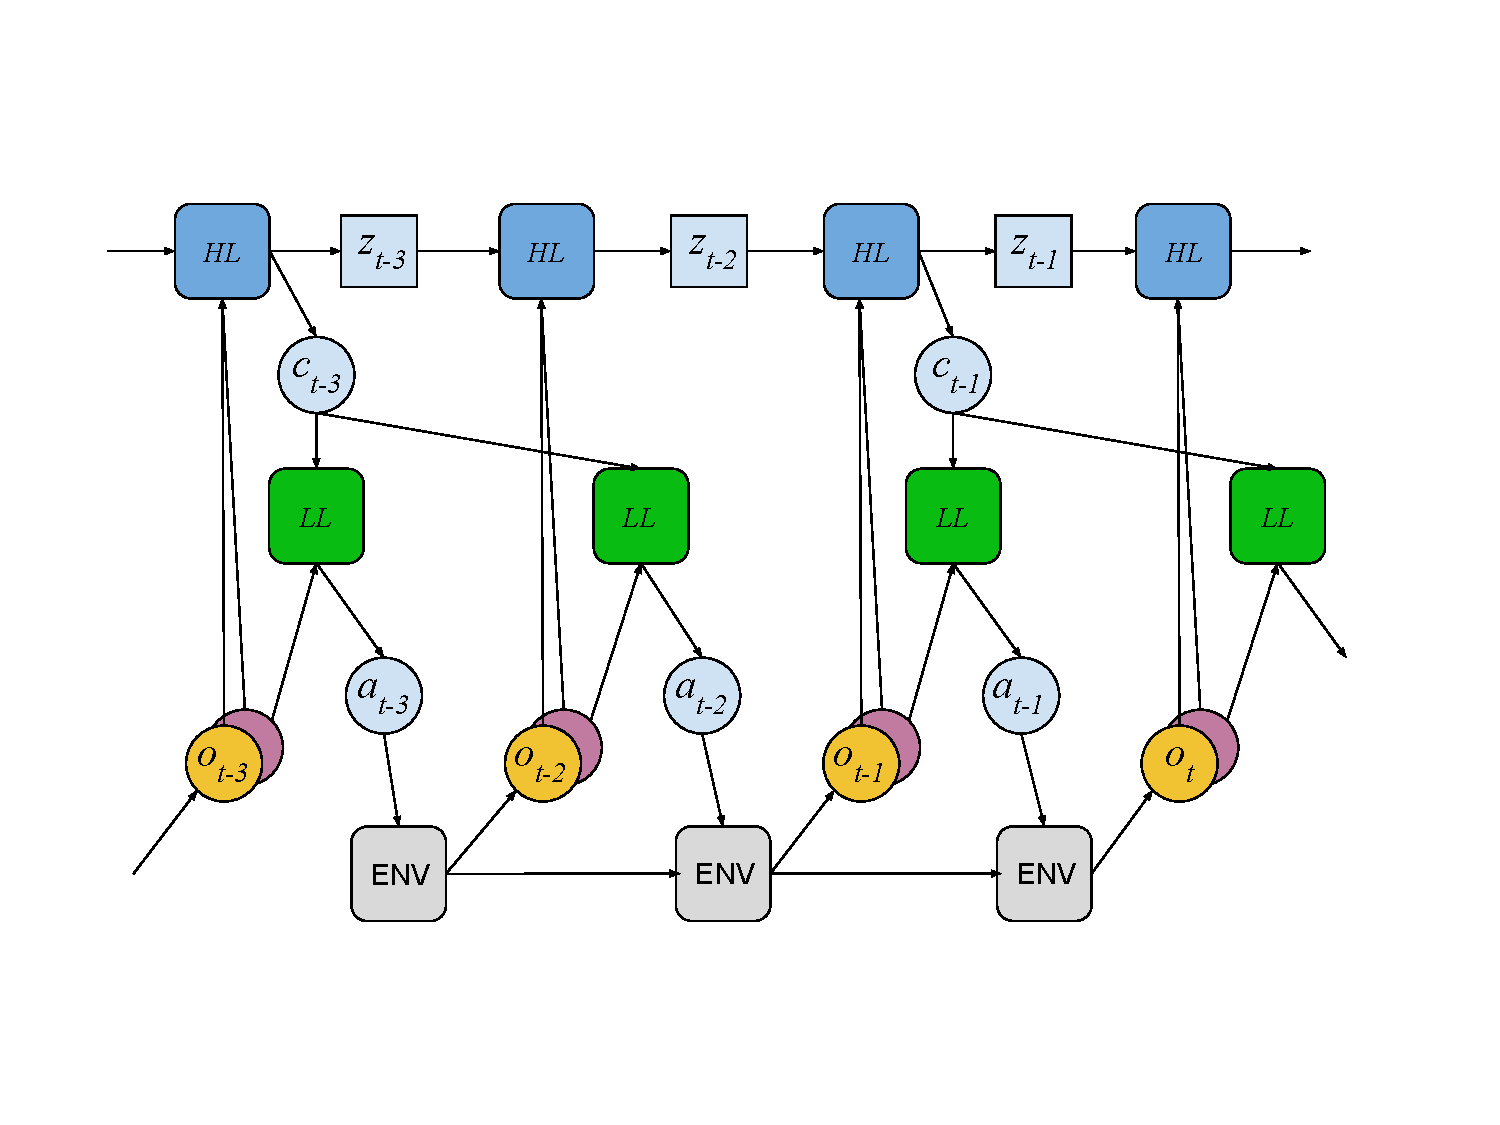
\includegraphics[width=\textwidth]{review_moduler_arch.pdf}
	\centering
	\caption{The hierarchical structure of the modulated controller~\cite{heess2016learning}, which consists
		of the recurrent high-level controller (HL, dark blue) and
		feedforward low-level controller (LL, green).  The
		high-level controller has access to all observations (yellow and red). While both controllers observe sensory
		input at the world-clock frequency, the modulatory con-
		trol signal from the high-level is updated every K
		steps (here K = 2)}\label{review_moduler_arch}
\end{figure}
The hierarchical agent is characterized by a policy $\pi$ with parameter $\theta$. The policy is defined by the composition of the high-level controller $F_H$ and low-level controller $F_L$. The low-level controller is a feed-forward neural network that maps the preprocessed curre
nt state $o(s)$ and the control signal from the high-level controller $c$ to the policy output.
\begin{align}
\pi (a| s) = F_L(o(s),c)
\end{align}
where the preprocessed state $o(s)$ removes task-specific information from the current state.
The high-level controller is a recurrent neural network: $F_H = (f_z,f_c)$ that produces the new control signal at every $K$ time step:
\begin{align}
z_t = f_z(s_t,z_{t-1}) \\
c_t = f_c(z_{t_r})
\end{align}
where $t_r$ is the most recent update output of the control signal. A predefined Gaussian noise component is added to the output $c_t$ during the training of the high level controller, so that the agent has a better performance in exploration.
The training of the hierarchical agent consists of two separate phases: pre-training and transfer. The tasks used for pre-training are relatively simple tasks that facilitate the development of generic locomotion skills. After pre-training, the high-level controller is re-initialized and the weights of low-level controller are frozen. The high-level controller is then trained in the transfer task, which has a sparse reward function.

This method manages to solve a few sparse problems with low-dimensional state inputs, which could not be solved by any flat reinforcement learning methods. The limitation is that the architecture requires heavy problem-specifc engineering components. The observation of the low-level agent $o(s)$ is designed manually. the hierarchical relationships between the two agent, including the definition of pre-training environments and the modulation model are also predefined. Apart from that, the low-level agent can only be executed for a predefined number ($K$) of time-steps before it gets terminated. This design could only be useful in a limited class of problems.

\subsection{Learning a hierarchical model by meta-learning}
Another work~\cite{frans2017meta}, namely meta learning shared hierarchies (MLSH), proposes a metalearning approach for learning hierarchically structured policies.
The MLSH method formulates the problem as learning a finite set of MDPs $P_M$ with the same state-action space, with a universal agent architecture. The agent consists of two sets of parameters $(\phi,\theta)$, where $\phi$ is the set of task-independent parameters and $\theta$ is the set of task-specific parameters. The meta-learning objective is to optimize the expected return during the agent's entire lifetime:
\begin{align}
\mathrm{maximize}_\phi \mathbb{E}_{M\sim P_M}[R]
\end{align}
The detailed structure of the agent is shown in Figure~\ref{review_mlsh_arch}. The architecture is also a two-level hierarchical reinforcement learning agent, the components $\phi_1,\phi_2,\dots$ are the parameters of the low-level agent policies (called sub-policies) shared across different tasks and $\theta$ is the parameters of the high-level agent of the current task. The policy of the high-level agent, namely master policy, samples an action at fixed periods and selects the sub-policy to be executed.
\begin{figure}[h]
	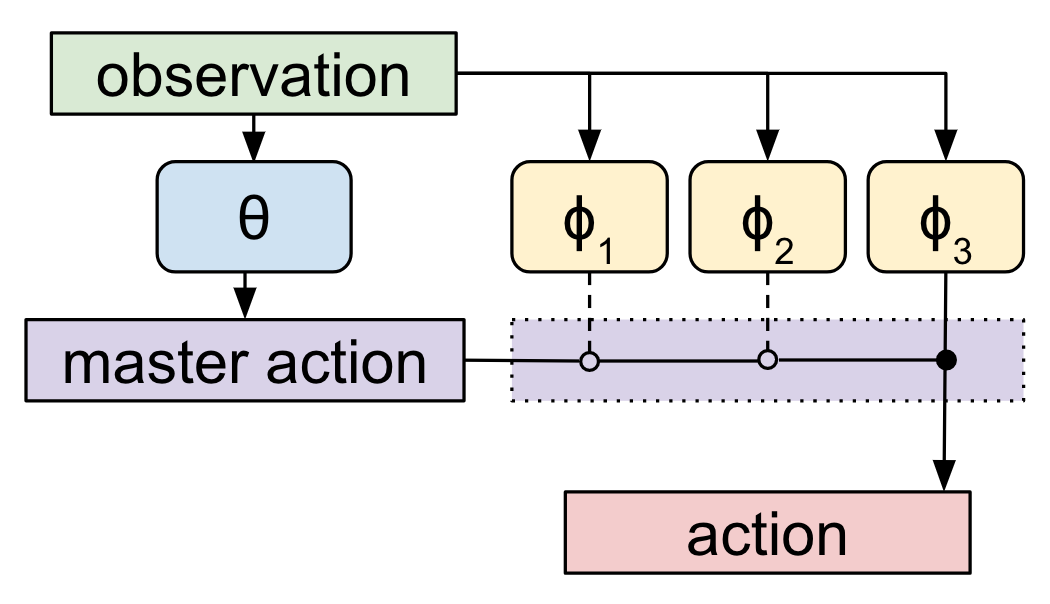
\includegraphics[width=0.5\textwidth]{review_mlsh_setup.png}
	\centering
	\caption{The agent setup of the modulated controller~\cite{frans2017meta},$\theta$ represents the master policy, which selects
		a sub-policy to be active. In the diagram, $\phi_3$ is the active sub-policy, and actions are taken according
		to its output.}\label{review_mlsh_arch}
\end{figure}
The agent is trained in the following manner: First a task is sampled $M$ is sampled and the parameter $\theta$ is re-initialized randomly. Then there is a warmup phase, where only $\theta$ is trained to achieve optimal. Then the agent enters the joint update phase, where both $\theta$ and $\phi$ are updated simultaneously.
The method achieves good performance in several control environments. Including a moving-bandit Ant-robot task, a Ant-robot maze navigation task and an obstacle course task. 

However the tasks are actually simplified version of the control tasks defined in \cite{duan2016benchmarking}. One modification is that the state of the "Ant" robot is periodically reset to prevent episode termination due to the falling over of the robot. The complexity of the task is thus largely reduced. It is not clear whether the method would perform well on the original version of the Ant environment.
The MLSH method also relies on a warm up period to learn the high-level agent's policy. However, the authors didn't provide a solution to learn the high-level agent's policy $\theta$ at the beginning where the parameter $\phi$ is also randomly initialized.
Finally also predefines the temporal relationship between the high level policy and low level policy, and the master agent only makes decision at pre-defined periods.
% \section{Hindsight Experience Replay}
% The work of~\cite{andrychowicz2017hindsight} generate actuator policies and there corresponding termination predicate policies based on the definition of subgoals. The subgoals are generated by heuristic functions of a target state. TODO
% \section{Scheduled Auxiliary Control}
% The work of \cite{riedmiller2018learning} proposes the method of scheduled auxiliary control. The method generates partial policy by a given set of simple auxiliary tasks, whose reward signals are generated based on heuristic functions of the sensor activation. The method also assume a constant execution length of the actuator policies. TODO
\subsection{Goal-directed learning method}
Several works~\cite{riedmiller2018learning}, ~\cite{andrychowicz2017hindsight} have attempted to solve sparse-reward robot control environments through the learning of auxiliary MDPs.
The method of~\cite{riedmiller2018learning}, namely Scheduled Auxiliary Control (SAC-X), is one of the representative works and is based on several main principles. First, the original MDP is modified, where the agent receives a vector reward signal at each timestep, consisting the reward for the original MDP and a set of internal auxiliary rewards. Second, each internal auxiliary reward function is assigned a low-level agent policy, namely intention. Third, there is a high-level agent that selects and executes the intentions. Fourth, the learning of intentions is performed off-policy on the same experience and is performed simultaneously for different intentions.
The definitions of internal auxiliary rewards are based on predefined goal states. The internal auxiliary reward with goal state $g$ is defined as:
\begin{equation}
r_g(s,a)=
\begin{cases}
\delta_g(s),& \text{if } d(s,g)\\
0,              & \text{else}
\end{cases}
\end{equation}
The parameter $\theta$ of the intentions is trained with the aggregation of loss of all the reward functions:
\begin{align}
\mathcal{L}(\theta)  = \mathcal{L}(\theta;M) +\sum_{k=1}^{|A|} (\mathcal{\theta;A_K})
\end{align}
Where $M$ is the MDP with the original reward function and $A=\{A_1,\dots,A_k\}$ is the set of MDPs with internal auxiliary rewards. The training of the intention parameter is formulated as a multi-task RL problem.
The high-level scheduler policy is the trained using an off-policy policy gradient method with $\theta$ being fixed.
The method manages to solve the object grasping and stacking problems in an robot-arm environment. 

One limitations of SAC-X is that the method relies on predefined auxiliary MDPs. Proposing auxiliary MDPs could be solved by heuristic algorithms in for some special problems, but is infeasible for general problems. Apart from that, the method limits the definition of auxiliary MDPs to be goal-directed task, which is impractical for high-dimensional realistic problems.


\subsection{Other methods targeting at sparse environments}
Apart from the above mentioned works, several other methods have also been proposed to solve environments with sparse reward recently, including Unicorn~\cite{mankowitz2018unicorn}, FuN~\cite{vezhnevets2017feudal},  HRL with Stochastic Temporal Grammar~\cite{shu2017hierarchical}, policy sketch method~\cite{andreas2016modular} and strategic attentive writer~\cite{vezhnevets2016strategic}. These methods are only verified in discrete environments and no evidence has shown that they are applicable to our target problem domains.

%!TEX program = xelatex
%!TEX root = ./thesis.tex
\chapter{Methodology}
%!TEX program = xelatex
%!TEX root = ./thesis.tex
\section{Target Environments}\label{sec_env}
\subsection{Summary of Environment Design}
We propose and develop a set of tasks that are representatives of deep reinforcement learning environments with continuous action space, multi-modal state space and sparse reward functions. The design of the robots' physical systems is based on the 3D robot environments~\cite{roboschool_2018} in OpenAI Gym~\cite{openaigym}. The external environments and reward functions of the target tasks are different from the original environments in OpenAI Gym. There are three classes of 3D robot agents in the environments OpenAI Gym: Ant, Humanoid and Swimmer. The Ant agent is a quadruped robot with 8-dimensional action space, the Humanoid agent is a humanoid robot with 16-dimensional action space, and the Swimmer agent is a worm-like robot with 2-dimensional action space.  The three agents are shown in Figure~\ref{fig_agent_ant}, Figure~\ref{fig_agent_humanoid} and Figure~\ref{fig_agent_swimmer}.

We mainly focus on a set of different problems based on the Ant agent, because the agent has the capability of solving a rich variety of high-level tasks, while the learning of the agent's basic control skills is not too challenging. 
Compared to the Ant agent, the Swimmer agent is too simple and its capability of solving hierarchical tasks is limited. The Humanoid agent, on the other hand, has a much more unstable physical system compared to Ant, and poses too much difficulty in the learning basic locomotion skills.
\begin{figure}[H]
	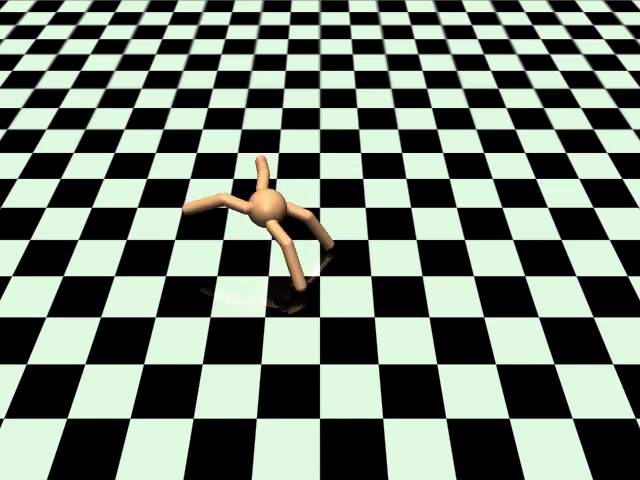
\includegraphics[width=0.5\textwidth]{images/agent_ant.png}
	\centering
	\caption{The Ant agent}\label{fig_agent_ant}
\end{figure}

\begin{figure}[H]
	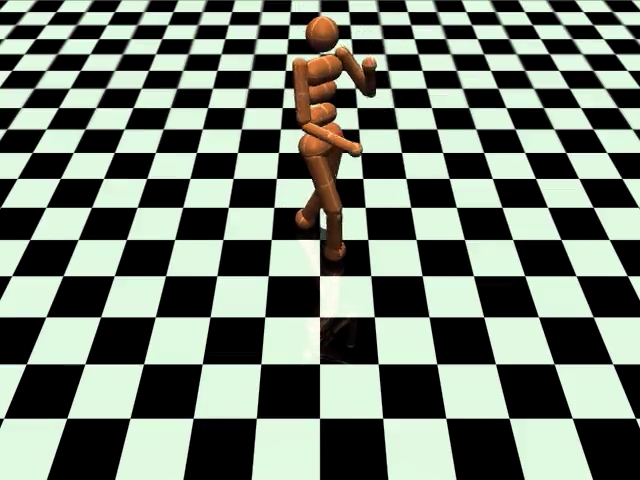
\includegraphics[width=0.5\textwidth]{images/agent_humanoid.png}
	\centering
	\caption{The Humanoid agent}\label{fig_agent_humanoid}
\end{figure}
\begin{figure}[H]
	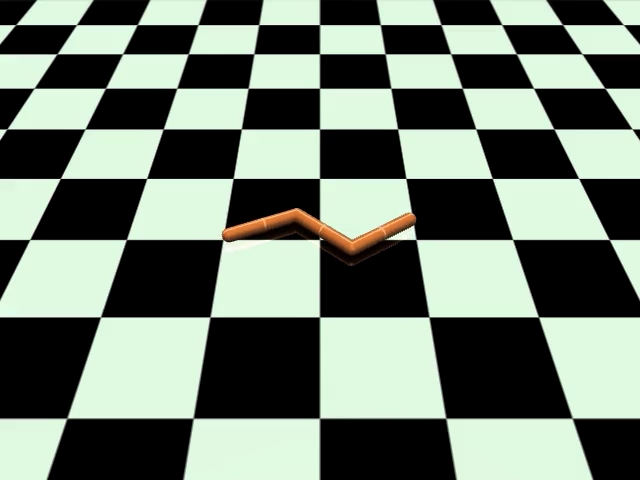
\includegraphics[width=0.5\textwidth]{images/agent_swimmer.png}
	\centering
	\caption{The Swimmer agent}\label{fig_agent_swimmer}
\end{figure}
%To provide a consistent comparison with other studies, the development of 
%!TEX program = xelatex
%!TEX root = ./thesis.tex

\subsection{Detailed Environment Specifications}
We provide a detailed description of the experiment environments in this section. All of the environments are based on the Ant task~\cite{openaigym}. 

In the original Ant task, the agent receives a 111-dimensional motion sensor input and produces an 8-dimensional action output. The input consists of a 13-dimensional vector that contains the robot's pose information, a 14-dimensional vector that represents its velocity information, and an 84-dimensional vector that contains contact force information. However, information about the agent's absolute position in the world map is not available.

For the proposed environments, the agent receives not only the 111-dimensional motion sensor input, but also a $64\times 64\times 1$ dimensional grayscale image observation. A sample image observation is shown in Figure~\ref{fig_ant_imgobs}. The image is not in a high resolution but is sufficient for the agent to observe the necessary information for the proposed tasks.

\begin{figure}[H]
	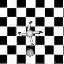
\includegraphics{images/ant_imgobs.png}
	\centering
	\caption{A sample image observation of the target environments}
\end{figure}\label{fig_ant_imgobs}

A basic task, namely move0, is similar to the Ant environment in OpenAI Gym~\cite{openaigym}. The difference is that the state space has an extra image input. The agent is required to move in a specific direction $g_0=(1,0)$, and the reward at each time-step is given by:
\begin{align}
r = v_g + 1-c_p-c_c
\end{align}
where $v_g=v \cdot g_0$ is the forward reward, which rewards the agent for moving in the target direction. A spherical object presents in the environments at a constant distance from the robot agent to represent the target direction.  $c_p$ is the control cost, which is the power that the agent is consuming, and $c_c$ is the contact cost, which penalizes the agent for collisions. The episode terminates when the agent enters the unrecoverable state of being upside-down, or if the episode length reaches 1000 time-steps.

Apart from move0, a set of similar tasks with different target directions are denoted as move1, move2, move3, ..., move7. These tasks are similar to move0 because the goal direction is different. The image observation is actually redundant for all these low-level tasks, because the agent only needs to move in one specific direction in their corresponding environments. Snapshots of these source tasks are shown in Figure~\ref{fig:task8}.
\begin{figure}[!htbp]
	\centering
	\begin{subfigure}[t]{0.3\textwidth}
		\centering
		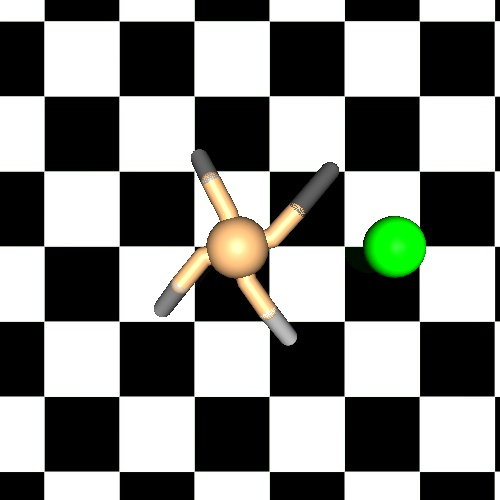
\includegraphics[width=\textwidth]{move0}
		\caption{move0}
	\end{subfigure}%
	~ 
	\begin{subfigure}[t]{0.3\textwidth}
		\centering
		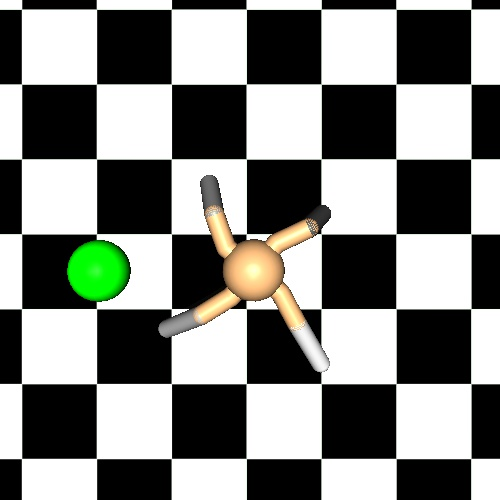
\includegraphics[width=\textwidth]{move1}
		\caption{move1}
	\end{subfigure}
	~ 
	\begin{subfigure}[t]{0.3\textwidth}
		\centering
		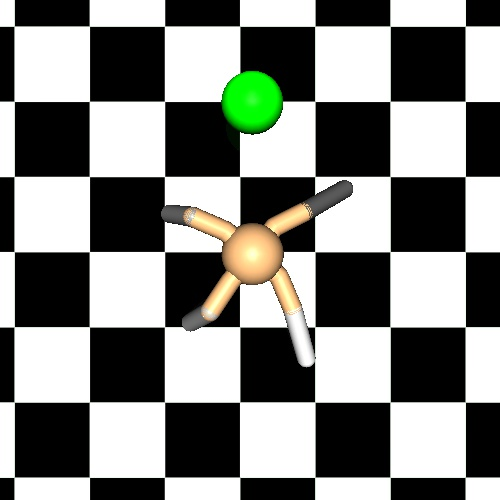
\includegraphics[width=\textwidth]{move2}
		\caption{move2}
	\end{subfigure}
	~ 
	\begin{subfigure}[t]{0.3\textwidth}
		\centering
		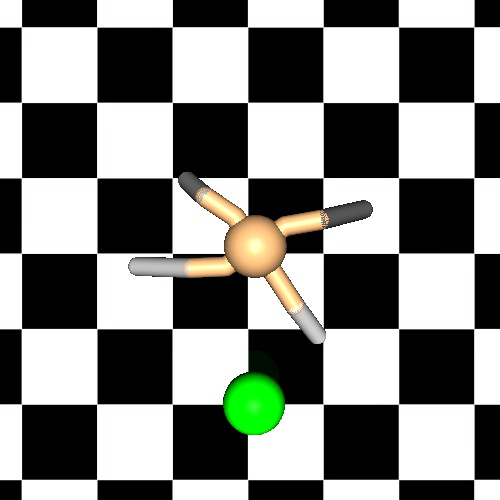
\includegraphics[width=\textwidth]{move3}
		\caption{move3}
	\end{subfigure}
	~ 
	\begin{subfigure}[t]{0.3\textwidth}
		\centering
		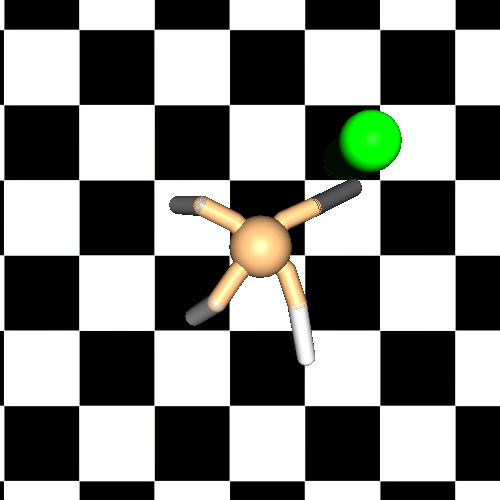
\includegraphics[width=\textwidth]{move4}
		\caption{move4}
	\end{subfigure}
	~ 
	\begin{subfigure}[t]{0.3\textwidth}
		\centering
		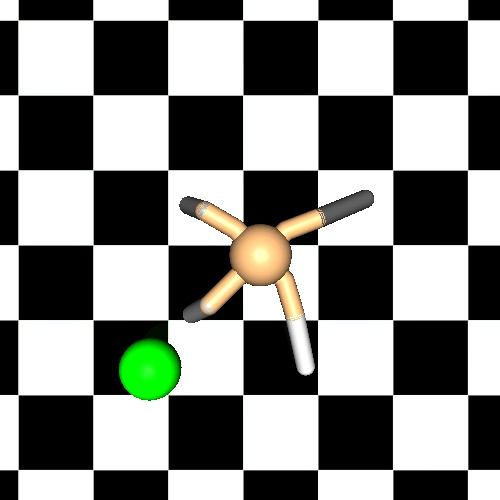
\includegraphics[width=\textwidth]{move5}
		\caption{move5}
	\end{subfigure}
	~ 
	\begin{subfigure}[t]{0.3\textwidth}
		\centering
		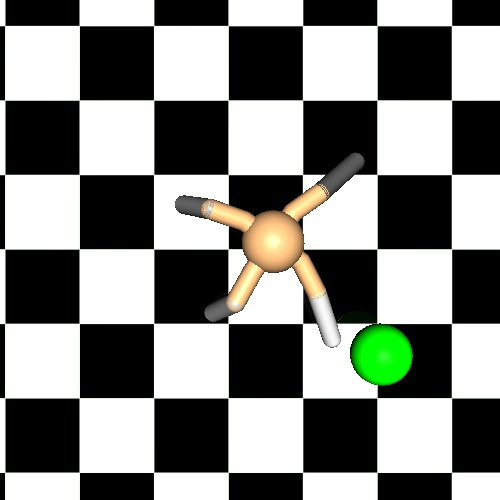
\includegraphics[width=\textwidth]{move6}
		\caption{move6}
	\end{subfigure}
	~ 
	\begin{subfigure}[t]{0.3\textwidth}
		\centering
		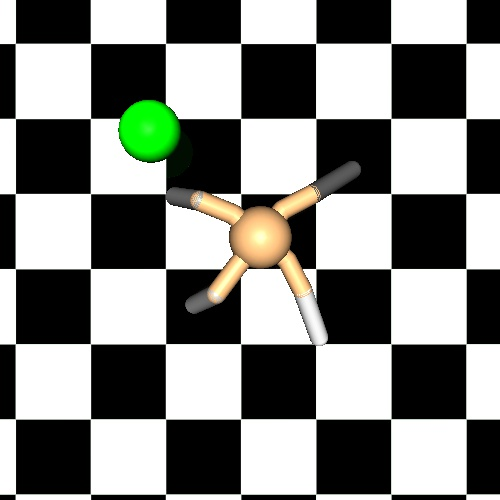
\includegraphics[width=\textwidth]{move7}
		\caption{move7}
	\end{subfigure}

	\caption{The source tasks}
	\label{fig:task8}
\end{figure}

Apart from these simple task, we also propose a set of tasks with more complexity. We propose several tasks with multi-modal state spaces such as moveg2, movecont, dynamicg8. These tasks require the agent to learn not only from the state representation but also the image representation. We also propose several more challenging tasks which has sparse reward fucntions, such as reachcont. The agent receives sparse reward signals in these environments. The target direction or location is represented by a spherical object and can be seen in the image observation.
The set of all the proposed environments are described in details in table \ref{table_ant_envs}.


\begin{table}[!htbp]

\begin{center}
\begin{tabular}{|c|p{3cm}|p{4cm}|p{4cm}|}
\hline
Task name & Goal & Reward  &  Description \\
\hline\hline
move0 & velocity: $g_0=(1,0)$ &$ v_g+1-c_p-c_c$  & move in a target direction \\
\hline
move1 & velocity: $g_1=(-1,0)$ &$ v_g+1-c_p-c_c$  & move in a target direction\\
\hline
move2 & velocity: $g_2=(0,1)$ &$ v_g+1-c_p-c_c$  & move in a target direction \\
\hline
move3 & velocity: $g_3=(0,-1)$ &$ v_g+1-c_p-c_c$  & move in a target direction \\ 
\hline 
move4 & velocity: $g_4=(\sqrt{2}/2,\sqrt{2}/2)$ &$ v_g+1-c_p-c_c$  & move in a target direction \\ 
\hline 
move5 & velocity: $g_5=(-\sqrt{2}/2,-\sqrt{2}/2)$ &$ v_g+1-c_p-c_c$  & move in a target direction \\ 
\hline 
move6 & velocity: $g_6=(\sqrt{2}/2,-\sqrt{2}/2)$ &$ v_g+1-c_p-c_c$  & move in a target direction \\ 
\hline 
move7 & velocity: $g_7=(-\sqrt{2}/2,\sqrt{2}/2)$ &$ v_g+1-c_p-c_c$  & move in a target direction \\ 
\hline 
moveg2 & velocity samples from: $\{g_0,g_1\}$ &$ v_g+1-c_p-c_c$  & each episode has a random sampled target direction \\ \hline
%moveg4 & velocity samples from: $\{g_0,g_1,g_2,g_3\}$ &$ v_g+1-c_p-c_c$  & each episode has a random sampled target direction \\ \hline
%moveg8 & velocity samples from: $\{g_0,g_1, \dots,g_7\}$ &$ v_g+1-c_p-c_c$  & each episode has a random sampled target direction \\ \hline
movecont & velocity samples from the unit circle&$ v_g+1-c_p-c_c$  & each episode has a random sampled target direction \\ \hline
dynamicg8 &  velocity samples from: $\{g_0,g_1, \dots,g_7\}$ &$ v_g$  & the target direction is re-sampled with probability 0.005 at each time-step  \\ \hline
%dynamiccont & velocity samples from a continuous range of all unit directions &$ v_g$  & the target direction is re-sampled with probability 0.005 at each time-step  \\ \hline
%reachg4 & position samples from $\{g_0,g_1,g_2,g_3\}$ & $I(\lVert x-g\rVert_2^2<0.5) - 0.01$  & The agent is terminated when reaching a target position\\ \hline
reachcont & position samples from the unit circle & $I(\lVert x-g\rVert_2^2<0.5) - 0.01$  & the episode is terminated when reaching a target position\\ \hline
reachcontreg & position samples from the unit circle & $5I(\lVert x-g\rVert_2^2<0.5) - 0.01$  & a new target is sampled and the episode continuous once the target position is reached\\ \hline
constdirreachreg & target direction samples from: $\{g_0,g_1, \dots,g_7\}$ & $5I(x_g > 1) - 0.01$  & a reward is given once the agent has moved in the target direction for a constant distance, then a new target is sampled\\ \hline
\end{tabular}
\end{center}
 \caption{Specification of the tasks}
\end{table}\label{table_ant_envs}




%!TEX program = xelatex
%!TEX root = ./thesis.tex
\section{Wasserstein Actor Critic Kronecker-factored Trust Region Policy Optimization Method }
As is reported in \cite{henderson2017matters}, the result of the current state-of-art deep reinforcement learning methods for continuous control, including TRPO, ACKTR, PPO and DDPG are difficult to be reproduced, due to they're heavily influenced by a variety of factors including random seed, neural network architecture, activation functions of neural network layers and even software implementation. This fact has reduced the reliability of these methods, and introduces difficulty in comparing their performance.

Particularly, the reproducibility problem with trust region methods including TRPO and ACKTR could be due to the training gets stuck in local minimum states. These trust region method has a naturally decreasing learning rate due to the KL-divergence measure. 

We propose a new policy optimization method, namely Wasserstein Actor Critic Kronecker-factored Trust Region Policy Optimization (W-KTR), in order to achieve a better performance on the proposed tasks, in terms of the agent's final performance, total training time and reproducibility.

The proposed W-KTR method focus on the problem scope of deep reinforcement learning for continuous control, specifically robot control problems. The physical meaning of action of these environments usually stands for mechanics-related physical quantity, such as motor torque and target motor phase. However, the traditional KL-divergence based trust region algorithms may not be suitable for these problems. Because the KL-divergence only focus on the intersection of policy distributions and may not be a good measure of the deviation of policy. A small perturbation in the mean value of a policy with Gaussian distribution from 1.0 to 1.01 will lead to a large KL-divergence when the variance has a small value such as 0.003. However, the perturbation may not lead to a significant difference in reality.

Therefore, we propose to use the Wasserstein metric, to measure the deviation of the policy updates. The Wasserstein metric as a trust region criteria has also been studied in previous literature~\cite{tolstikhin2017wasserstein}. We reformulate the trust region policy optimization problem as follows:
\begin{equation}
    \begin{aligned}
&    \underset{\theta}{\text{maximize}} 
&& J(\theta) \\
& \text{subject to } 
&& \overline{W_2}(\pi_{\theta_{old}},\pi_\theta) \leq \delta_{W}\end{aligned}
\end{equation}
where $ \overline{W_2}(\pi_{\theta_{old}},\pi_\theta)$ is the average Wasserstein-2 metric between the old policy and the current policy.

The Wasserstein-2 metric is defined by the following equation \cite{villani2003topics}:
\begin{equation}
    W_2(P,Q) = 
    \inf_{\Gamma \in \mathbb{P}(X \sim P, Y \sim Q)}
    \mathbb{E}_{X,Y \sim \Gamma} \left[ \lVert X-Y \rVert_2^2 \right]^{1/2}
\end{equation}
where $\mathbb{P}(X \sim P, Y \sim Q)$ is the set of all joint distribution of $X,Y$ with marginals $P,Q$ respectively.

Specifically, when $P$ and $Q$ are Gaussian distributions with mean $m_1,m_2$ and covariance matrix $\Sigma_1$ and $\Sigma_2$, the squared value of Wasserstein-2 distance $W_2^2(.)$ is defined as the following equation~\cite{chafai} :
\begin{equation}
    W_2^2(P,Q) = \Vert m_1-m_2\Vert_2^2 +\mathrm{Tr}\left(\Sigma_1+\Sigma_2-2(\Sigma_1^{1/2}\Sigma_2\Sigma_1^{1/2})^{1/2}\right)
\end{equation}

The problem is solved by performing gradient updates iteratively following the natural gradient with the Rianmanian metric as $W_2$ metric:

\begin{equation}
    s=H_\theta\left( \overline{W_2^2}(\pi_{old},\pi) \right)^{-1}g := A^{-1}g
\end{equation}
%
%We use the approximation of the Rianmanian metric tensor A:
%
%\begin{equation}
%    A \approx \mathbb{E}_{s_t} \left[
%    \nabla_\theta W_2^2(\pi_{old},\pi) \left(\nabla_\theta W_2^2(\pi_{old},\pi) \right)^T
%    \right]
%\end{equation}
If the non-diagonal entries in covariance matrices are all zero, the metric $W_2^2(.)$ is simply a second order term over the means and the square root of the covariance matrices:
\begin{equation}
W_2^2(P,Q) = \Vert m_1-m_2\Vert_2^2 +\Vert \Sigma_1^{1/2}-\Sigma_2^{1/2}\Vert_2^2
\end{equation}
The metric can actually be represented as a squared error between two parameter vectors:
\begin{equation}
W_2^2(P,Q) = \Vert \text{vec}[m_1,diag(\Sigma_1^{1/2})]-\text{vec}[m_2,diag(\Sigma_2^{1/2})]\Vert_2^2 
\end{equation}
The solution of this kind of expressions can then be computed using the Kronecker-factor approximation technique~\cite{wu2017scalable}.

The policy is then updated following the gradient direction $s$ with ADAM stochastic optimization algorithm~\cite{kingma2014adam}. The step size is adjusted in an adaptive manner according to the resulting $W_2$ distance at each training step.
%!TEX program = xelatex
%!TEX root = ./thesis.tex
\section{Efficient Exploration Through Exceptional Advantage Regularization}\label{sec_method_expadv_reg}
One of the challenges with multi-modal state-space robot environments is to simultaneously learn features from different sources of state inputs.

The state spaces of the studied problems have two modalities: the locomotion sensor signal and the image observation. The complexity in learning the features from the two inputs is different. The learning of motion sensor signal features is usually trivial while the learning of image features takes much more time. The agent would get stuck at a local minimum after it has learned the features of the locomotion state vectors but still without learning anything from the image input.

As far as we know, the distribution type of the continuous stochastic policy in reinforcement learning is usually chosen to be a normal distribution with diagonal covariance matrices in the previous studies of on-policy policy gradient methods. We have observed a phenomenon in the training process of policy gradient methods that, the variance of policy is extremely unlikely to be increased, even when the agent has just escaped from a local minimum. This phenomenon leads to inefficiency in exploration. Therefore, a regulation method is necessary to encourage the agent to perform exploration without hurting the reinforcement learning performance.

A conventional regularization method to encourage exploration is entropy regularization:

\begin{align}
g' = g +\beta_{ent}\nabla_\theta \mathbb{E}[ H(\pi_\theta(a|s)) ]
\end{align}
where $\beta_{ent}$ is the weight controlling the penalty on low entropies.
The entropy of a normal distribution $\mathcal{N}(\mu,\Sigma)$ is defined as:

\begin{align}
	H(\pi) =  \frac{1}{2} \ln \mathrm{det}(2\pi e \Sigma)
\end{align}

If the policy distribution is a normal distribution with diagonal covariance matrix, the entropy regularization basically introduces a constant bias to the gradient of the logarithm of variance parameters. As a result, the entropy regularization method is usually hard to tune so that the agent can efficiently perform exploration without significant degradation in the reinforcement learning performance.

We propose a novel method, namely  Exceptional Advantage Regularization, that can encourage exploration. We add a term, namely Exceptional Advantage Regularization loss (EAR), to the gradient of the variance parameters:
\begin{align}
g'_\Sigma = g_\Sigma + \beta_{ex} \mathbb{E}_{\hat{A}^{GAE}(s) > 0} \left[
\hat{A}^{GAE}(s) 
\max\left(0,\nabla_\Sigma \log \pi (a|s)\right)\right]
\end{align}
%\begin{align}
%g'_\Sigma = g_\Sigma + \beta_{exc} \mathbb{E} \left[
%	\max\left(0,I(\hat{A}^{GAE}>0) \hat{A}^{GAE} \nabla_\Sigma \log \pi (a|s)\right)\right]
%\end{align}
where $\beta_{ex} $ is the weight controlling the bias on exploration.

The EAR loss adds a bias for the positive gradients of the variance parameters of the samples with positive advantage values. By introducing the EAR loss, more importance is added to the samples with low likelihood which produce exceptionally positive advantage values. As a result, the positive experiences that are rarely encountered would be paid more attention. The problem remaining is to identify the samples with low likelihood. We simply take the positive gradients of the variance parameters with respect to the log-likelihood here to filter out the samples whose likelihoods are too high.

%!TEX program = xelatex
%!TEX root = ./thesis.tex
\section{Efficient Exploration Through Robust Concentric Gaussian Mixture Policy}
Apart from the EAR method for exploration, we propose to use an alternative probability distribution type, namely Robust Concentric Gaussian Mixture, instead of a diagonal Gaussian policy used in previous works.

The proposed policy distribution, namely Robust Concentric Gaussian Mixture (RCGM) Policy, is a mixture of two Gaussian distributions,
\begin{align}
\pi (a|s) = (1-\alpha_{ex})\mathcal{N}(\mu,\Sigma) + \alpha_{ex} \mathcal{N}(\mu,q_{ex}\Sigma)
\end{align}
where the constant $\alpha_{ex}$ is the weight of second distribution. The weight $\alpha_{ex}$ can take a value in the range of $(0,1)$, such as $0.05$, and the constant $q_{ex} \in (1,)$, for example can be $5$, controls the variance of the second deviation. The larger $q_{ex}$ is, the higher the likelihood will be in the tails of the distribution. The resulting distribution actually has the same number of trainable parameters as the first component, since both $\alpha_{ex}$ are set to fixed parameters.

The KL-divergence of two RCGM policy does not have a closed form expression even for this special case. An empirical estimation can be used to approximate the KL-divergence ~\cite{hershey2007approximat}:%TODO: fix citation
\begin{align}
KL(p, q) \approx\mathbb{E}_{x\sim p} \log [ \left(p(x)/q(x)\right) ]
\end{align}

However, an empirical estimation of the KL-divergence can still be computed based on the training samples. Apart from that, the Wasserstein-2 distance between two RCGM policy can be given by:
\begin{align}&W_2^2(\pi_{0}(a|\mu_0,\Sigma_0), \pi_{1}(a|\mu_1,\Sigma_1) =  \\ \nonumber
& \ \ \ \ (1-\alpha_{ex})
W_2^2\big(\mathcal{N}(\mu_0,\Sigma_0), \mathcal{N}(\mu_1,\Sigma_1)\big)
+ \alpha_{ex} W_2^2\big(\mathcal{N}(\mu_0,q_{ex}\Sigma_0), \mathcal{N}(\mu_1,q_{ex}\Sigma_1)\big)
\end{align}


Compared to the commonly used Diagonal Gaussian distribution, the RCGM distribution could be much more robust since it has longer tails. Therefore, it is less likely that the agent gets stuck at sub-optimal policies.


\section{Hierarchical reinforcement learning architecture}
We propose to solve the reinforcement learning problem by a two-level hierarchical model. 

The hierarchical model consists of a top-level decider agent and a set of bottom-level actuator agents. The actuator agents' policies are trained im the source task environments. 

The decider agent takes an action at every time-step. It may either decide which actuator-policy should be executed, or simply skip and continue current actuator-policy. Therefore, assume there are $n_a$ sub-policies, the action space of the root agent is an $(n_a+1)$-discrete action space.

The observation space of the root agent consists of 2 parts, original statn (motion-sensor observation, image observation) and the meta state. The meta observation state the current sub-policy being executed and the number of time-steps since the last decision has been made.

Empirically, the decider agent is parameterized by two policy networks, $\theta_s$ and $\theta_d$. The network $\theta_s$, namely switcher network, outputs a binary action that decides whether the agent should simply continue using the current acting actuator policy, or switch to another policy based on the current state. The agent

The network $\theta_d$, namely decider network, outputs an $n_a$-discrete action space, that select the acting agent

The selected leaf agent executes the corresponding sub-policy and computes the primary actions the agent should take for the original environment.

 The overalll decision-making process of the decider agent is shown in Algorithm~\ref{hrl_decision_proc}.

\begin{algorithm}
\caption{The decider agent mechanism}\label{hrl_decision_proc}
\begin{algorithmic}%[1]
\Function{deciderAct}{self,$s_t$}
\State $a_{decider} \sim \pi_{decider}(s_t)$
 \If{$a_{decider} \neq 0$}
 \State $self.currentActuator \gets self.allA
ctuators[a_{decider}-1]$
 \EndIf
\State $a_{actuator} \gets self.currentActuator.act(s_t)$
\State \Return $a_{actuator}$
\EndFunction
\end{algorithmic}
\end{algorithm}


\section{Generalized advantage estimation for hierarchical reinforcement learning agents}
We propose a generalized advantage estimation method for decider agents hierarchical reinforcement learning agents. 

Assume that a decider agent makes decisions at time $t_1,t_2,\dots$, then the execution length of the decisions are $l_i = t_{i+1} - t_i, i=1,2,\dots$.

Then the definition of reward of the decider action at $t_i$ is given by:
\begin{align}
\bar{r}_{t_i} \defeq
 \sum_{l=0}^{t_{i+1}-t_i-1}
  \gamma^l r_{t_i+l}
\end{align}

Define the TD residual $\dv_{t_i}$ for $i=0,1, \dots$by:
\begin{align}
\dv_{t_i} & \defeq -V(s_{t_i}) + \bar{r}_{t_i} + \gamma^{t_{i+1}-t_i} V(s_{t_{i+1}})
\end{align}
Then the k-step advantage estimation is given by:
\begin{alignat}{2}
\hata_{t_i}^{(1)} 
& \defeq   \dv_{{t_i}} 
 &&=-V(s_{t_i}) + \bar{r}_{t_i} + \gamma^{t_{i+1}-t_i} V(s_{t_{i+1}})\\
\hata_{t_i}^{(2)} 
&\defeq \dv_{t_i} + \gamma^{t_{i+1}-t_i} \dv_{t_{i+1}} 
&&= -V(s_{t_i}) +\bar{r}_{t_i} + \gamma^{t_{i+1}-t_i} \bar{r}_{t_{i+1}} + \gamma^{t_{i+2}-t_i} V(t_{i+2}) \\
\hata_t^{(3)} 
&\defeq \dv_{t} + \gamma \dv_{t+1} + \gamma^2 \dv_{t+2} 
&&= -V(s_t) + r_t + \gamma r_{t+1} + \gamma^2 r_{t+2} + \gamma^3 V(s_{t+3}) \label{a3}
\end{alignat}
\begin{align}
\begin{split}
\hata_{t_i}^{(k)} 
&\defeq \sum_{d=0}^{k-1} 
\gamma^{t_{i+d}-t_i} \dv_{t_{i+d}} \\
&= -V(s_t) 
+\bar{r}_{t_i} + \gamma^{t_{i+1}-t_i} \bar{r}_{t_{i+1}} 
+ \dots 
+ \gamma^{t_{i+k-1}-t_i} \bar{r}_{t_{i+k-1}} 
+ \gamma^{t_{i+k}-t_i} V(s_{t_{i+k}})
\end{split}
\end{align}
We can define the unnormalized generalized advantage estimator as a exponentially-weighted sum of these k-step advantage estimators~\cite{schulman2015high}:
\begin{align}
\hata_{t_i}^{GAE_{unnorm}(\lambda)}
&\defeq  \hata_{t_i}^{(1)} + \lambda^{t_{i+1}-t_i}  \hata_{t_i}^{(2)} + \lambda^{t_{i+2}-t_i} \hata_{t_i}^{(3)} + \dots + \lambda^{t_{i+k-1}-t_i} \hata_{t_i}^{(k)} \nonumber \\
&=  \dv_{t_i} 
+ \lambda^{t_{i+1}-t_i} (\dv_{t_i} + \gamma^{t_{i+1}-t_i} \dv_{t_{i+1}} ) \\
&\ \ \ \ \  \ \ \ \ \ \ +\lambda^{t_{i+2}-t_i} (\dv_t + \gamma^{t_{i+1}-t_i} \dv_{t_{i+1}} + \gamma^{t_{i+2}-t_i} \dv_{t_{i+2}}) + \dots \nonumber \\
&\ \ \ \ \  \ \ \ \ \ \ +\lambda^{t_{i+k-1}-t_i}  \sum_{d=0}^{k-1} \gamma^{t_{i+d}-t_i} \dv_{t_{i+d}}\\
&= (
\dv_{t_i}  \sum_{b=0}^{k-1} \lambda^{t_{i+k-1}-t_i}
+\gamma^{t_{i+1}-t_i} \dv_{t_{i+1}} \sum_{b=1}^k \lambda^{t_{i+b}-t_i} \nonumber \\
&\ \ \ \ \  \ \ \ \ \ \ +\gamma^{t_{i+2}-t_i} \dv_{t_{i+2}} \sum_{b=2}^k \lambda^{t_{i+b}-t_i}
+\dots \\
&\ \ \ \ \  \ \ \ \ \ \ +\gamma^{t_{i+k-1}-t_i} \dv_{t_{i+k-1}} \lambda^{t_{i+k-1}-t_i})
\nonumber \\
&= \sum_{d=0}^{k-1} \dv_{t_i} \gamma^{t_{i+d}-t_i} \sum_{b=0}^{k-1} \lambda^{t_{i+b}-t_i}
\label{eq:gaelam1}
\end{align}
The normalized generalized advantage estimater is then given by:
\begin{align}
\hata_{t_i}^{GAE(\lambda)}
= \frac{\hata_{t_i}^{GAE_{unorm}(\lambda)}}{\sum_{b=0}^{k-1} \lambda^{t_{i+b}-t_i}}
\end{align}
However, the unormalized GAE estimator is usually used in practice instead of the normalized one, with a postprocessing step of batch normalization to adjust the scale of the advantages. This pratical method usually lead to large advantage scales for experience data at the beginning of the episodes and small scales for the experience data near episode ends.


%!TEX program = xelatex
%!TEX root = ./thesis.tex
\chapter{Experiments}

%%!TEX program = xelatex
%!TEX root = ./thesis.tex
\section{Solution to the basic environment: \textit{move0}}
In this section, we compare the proposed W-KTR method with other state-of-art algorithms on the basic \textit{move0} environment.

The performance of W-KTR algorithm is shown in Figure \ref{rec_move0_wktr_tune}:

\begin{figure}[h]
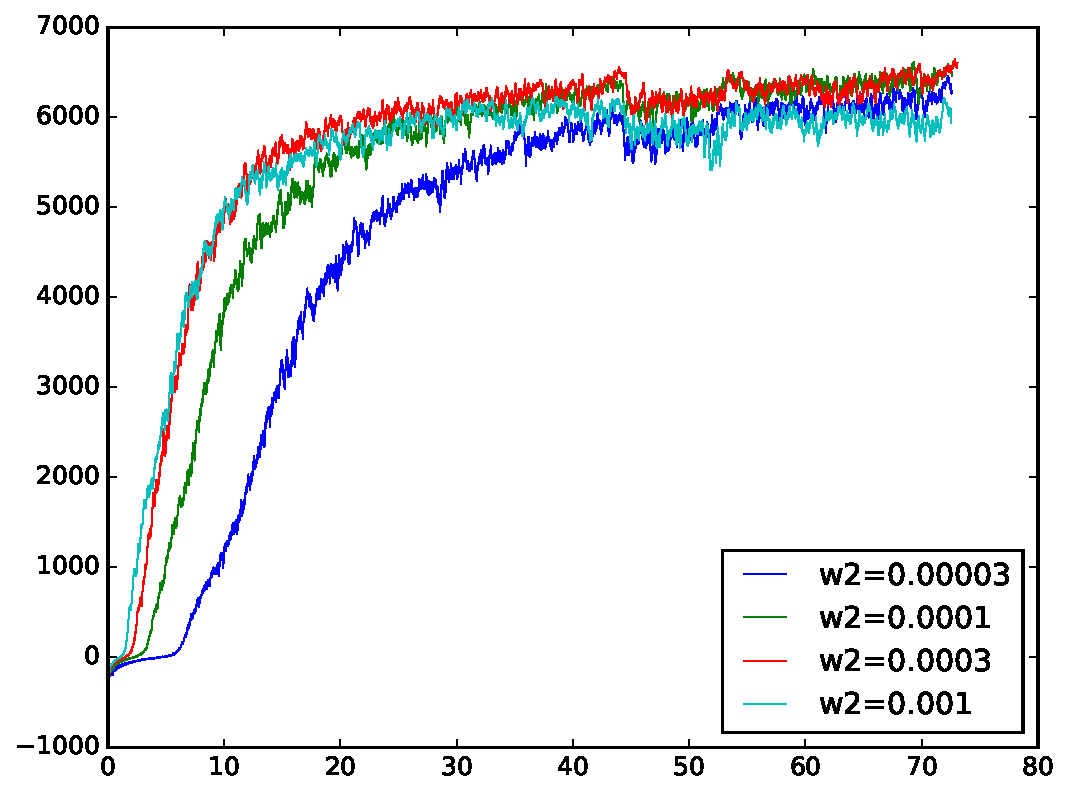
\includegraphics[width=\textwidth]{images/rec_move0_wktr_tune.pdf}
\centering
\caption{Performance of move0 W-KTR agent with diferent hyper-parameter $\delta_W^2$, the x-axis is the number of million timesteps and the y-axis is the total episode reward averaged over the last 200 episodes}
\end{figure}\label{rec_move0_wktr_tune}
It can be shown that the W-KTR agent has a stable final performance, which is not much dependent on the hyper-parameter $\delta_W^2$.

The performance of ACKTR agents is shown in Figure \ref{rec_move0_acktr_tune}:
\begin{figure}[h]
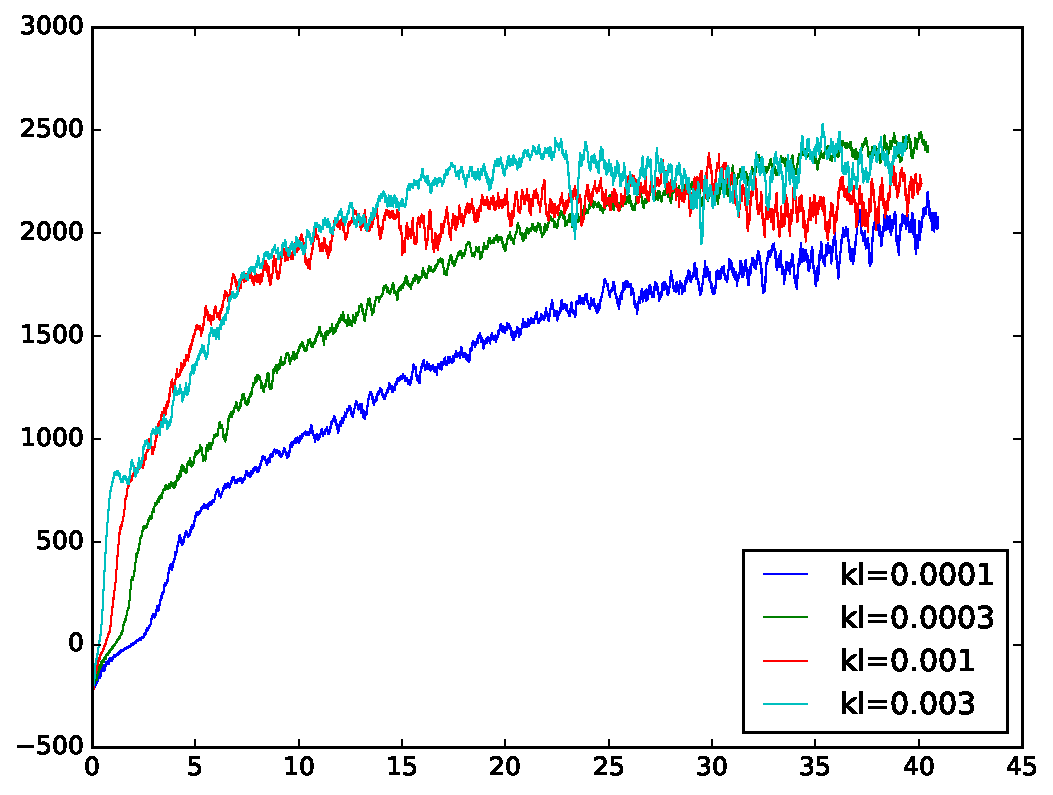
\includegraphics[width=\textwidth]{images/rec_move0_acktr_tune.pdf}
\centering
\caption{Performance of move0 PPO agent with diferent hyper-parameter $\delta_{kl}$, the x-axis is the number of million timesteps and the y-axis is the total episode reward averaged over the last 200 episodes}
\end{figure}\label{rec_move0_acktr_tune}
It can be shown that the ACKTR agent can achieve a faster rate of improvement at the first 10 million steps, but the improvement rate becomes slow as the training proceeds. The agents tend to stuck at sub-optimal policies since the policies converge too fast and cannot effectively adjust once the STD becomes small.

We also run experiments on tuning a PPO agent for the task move0, which is shown in Figre~\ref{rec_move0_ppo_tuning}. The original PPO algorithms has 40 minibatch updates in each batch, which converges too early. We only performa one gradient update over the whole batch in this experiment. The performance of the PPO agent appears to be sensitive to the hyper-parameter, and the agent can't avoid the drop of performance in the late phase of training. The method also needs to trade-off between the early improvement rate and the final performance. In conclusion, the PPO method is not a robust algorithm.
\begin{figure}[h]
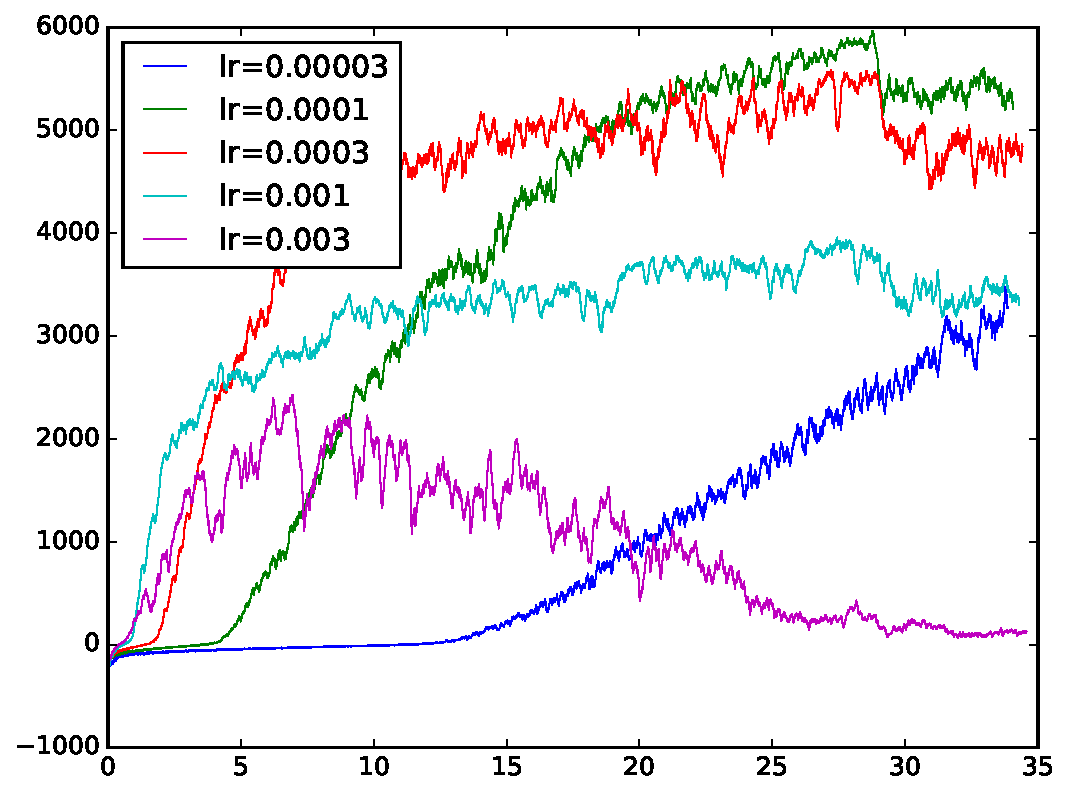
\includegraphics[width=\textwidth]{images/rec_move0_ppo_tuning.pdf}
\centering
\caption{Performance of move0 PPO agent with diferent hyper-parameter $learning rate$, the x-axis is the number of million timesteps and the y-axis is the total episode reward averaged over the last 200 episodes}
\end{figure}\label{rec_move0_ppo_tuning}

All the method above use a batch size of 4000 timesteps produced by 20 parallel agents.

\section{Flat solution to a simple Multi-Modality environment: \textit{move1d}}
In the move1d environment, the agent needs to learn from the image input to decide whether to move forward or backward, as well as control according to the states.
We have tried to solve the problem using ACKTR method, presented in Figure~\ref{rec_flatmove1d_acktr_tune}, shows that the agent can easily get stuck at the score of 1000, and cannot improve much even if the agent breaks the bottleneck because the average STD parameter already drops to below 0.04.
\begin{figure}[h]
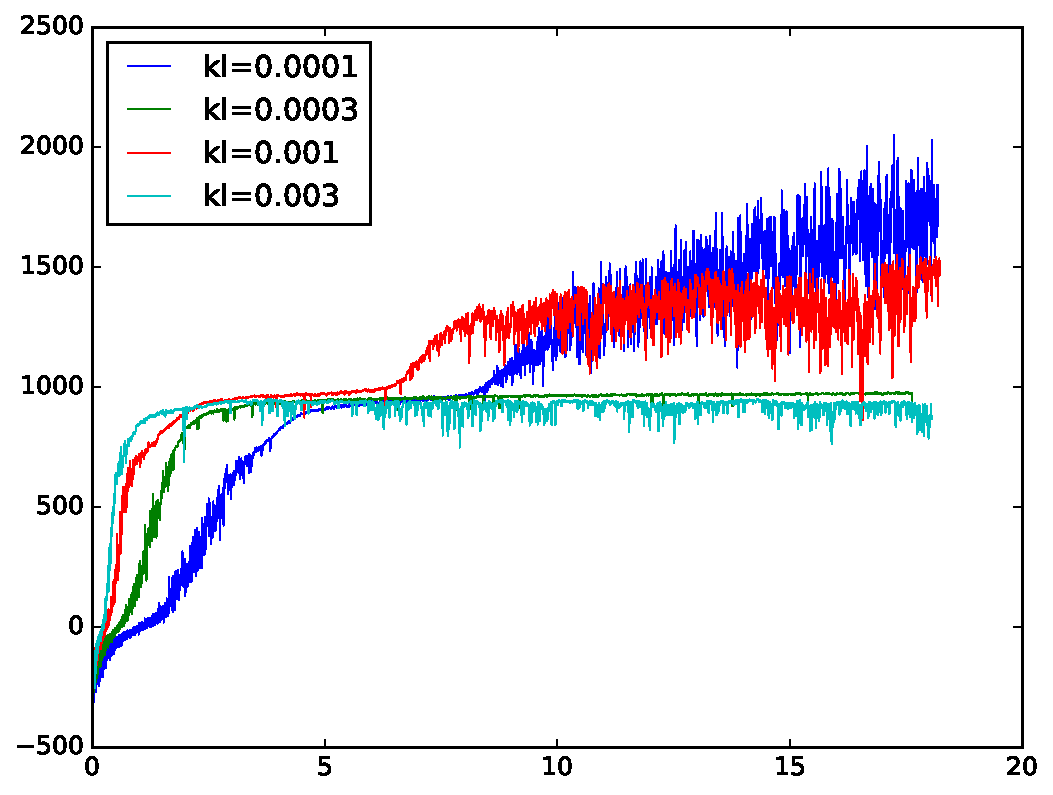
\includegraphics[width=\textwidth]{images/rec_flatmove1d_acktr_tune.pdf}
\centering
\caption{Performance of move1d ACKTR agent with diferent hyper-parameter $learning rate$, the x-axis is the number of million timesteps and the y-axis is the total episode reward averaged over the last 20 episodes}
\end{figure}\label{rec_flatmove1d_acktr_tune}

We also did a single experiment using the proposed W-KTR method, and is shown in Figure~\ref{rec_flatmove1d_wktr}. The W-KTR agent manages to achieve a fast improvement rate and high final performance after getting stuck at the bottleneck score 1000 for a while.
\begin{figure}[h]
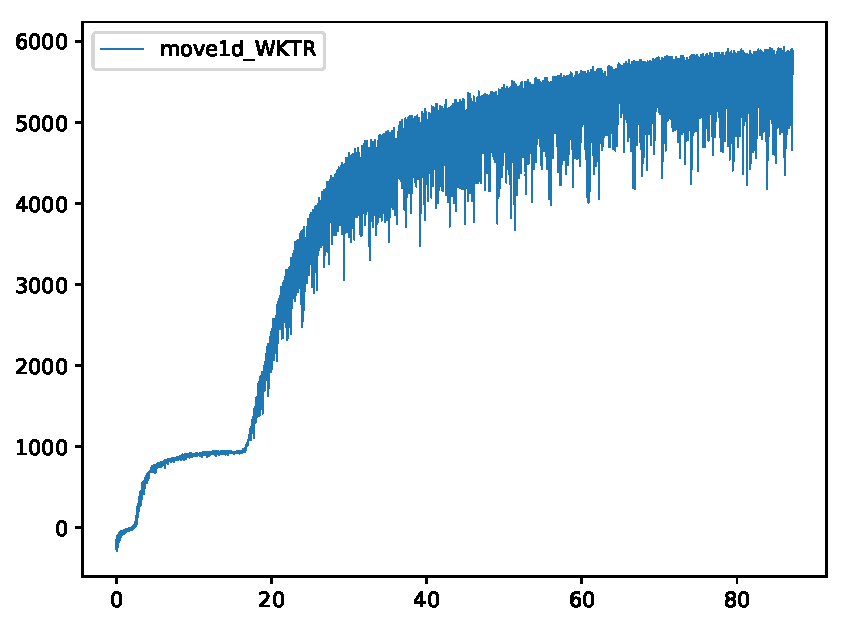
\includegraphics[width=\textwidth]{images/rec_flatmove1d_wktr.pdf}
\centering
\caption{Performance of move1d W-KTR agent with  hyper-parameter $\delta_W^2= 0.0001$, the x-axis is the number of million timesteps and the y-axis is the total episode reward averaged over the last 20 episodes}
\end{figure}\label{rec_flatmove1d_wktr}

This proves that the W-KTR agent is better at handle local minimum and re-adjust the agent's policy even when the policy STD becomes low.



%!TEX program = xelatex
%!TEX root = ./thesis.tex

\section{Experiment on the flat reinforcement learning solution to multi-modality tasks}
\subsection{Discussion on conventional flat reinforcement learning methods}
We observe contemporary end-to-end flat reinforcement learning methods fail to achieve good performance. We suggest that one of the important reason is the image features are much harder to learn than the state. The agent would tend to stuck at a local minimum when it has already learned the state features well, but has not been able to extract any useful information from the image. However, when the agent has finally learned the image features, the policy already converge to a relatively low-entropy distribution, and contemporary reinforcement learning methods cannot perform exploration again at this phase.

We take the task "movecont" as an example. In this task, a goal direction as sampled uniformly at random from the continuous range of angles: $[0,2\pi)$, at the beginning of each episode. The agent can only indicate the goal direction from the image, where there is a sphere object at the corresponding position.

A conventional method for encouraging exploration of reinforcement learning agents with continuous action space is entropy regularization. As we discussed in the section~\ref{sec_method_expadv_reg}, the entropy regularization method is not an effective method in the general case because it simply adds constant biases on the policy parameters and may dominate the learning of the original task.

An experiment on the effectiveness of entropy regularization is shown in Figure~\ref{rec_ent_reg}. The agents are trained using ACKTR algorithm with 32 parallel agents, minibatch-size 2560 and KL-divergence constraint 0.0003. The result shows that the agent easily fails to learn the original task when the weight on entropy term is too large. 

The change of average Standard Deviation of the policy distributions is shown in Figure~\ref{rec_std_ent_reg}. The agents' policy distributions appear to get stuck at certain level of standard deviation when the entropy term is not optimal.
\begin{figure}[!htbp]
	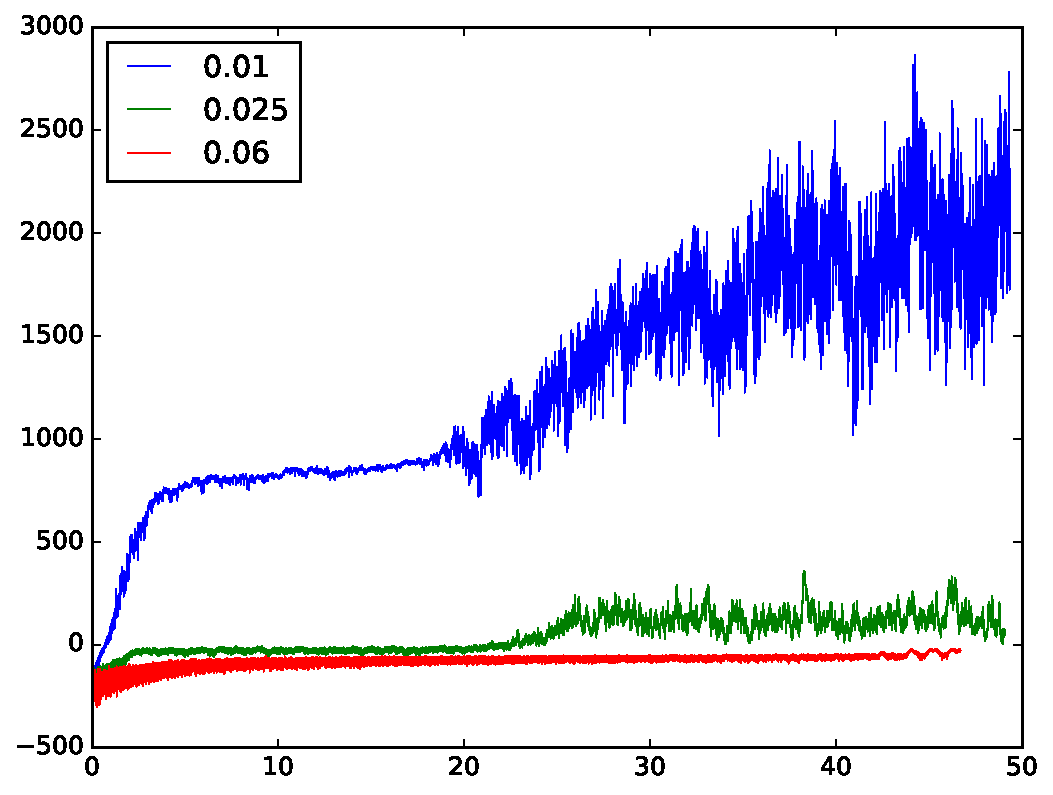
\includegraphics[width=\textwidth]{images/rec_ent_reg.pdf}
	\centering
	\caption{Performance of agents with different weight on entropy regularization term, the horizontal axis is the number of million timesteps and the vertical axis is the total episode reward averaged over the last 32 episodes}\label{rec_ent_reg}
\end{figure}

\begin{figure}[!htbp]
	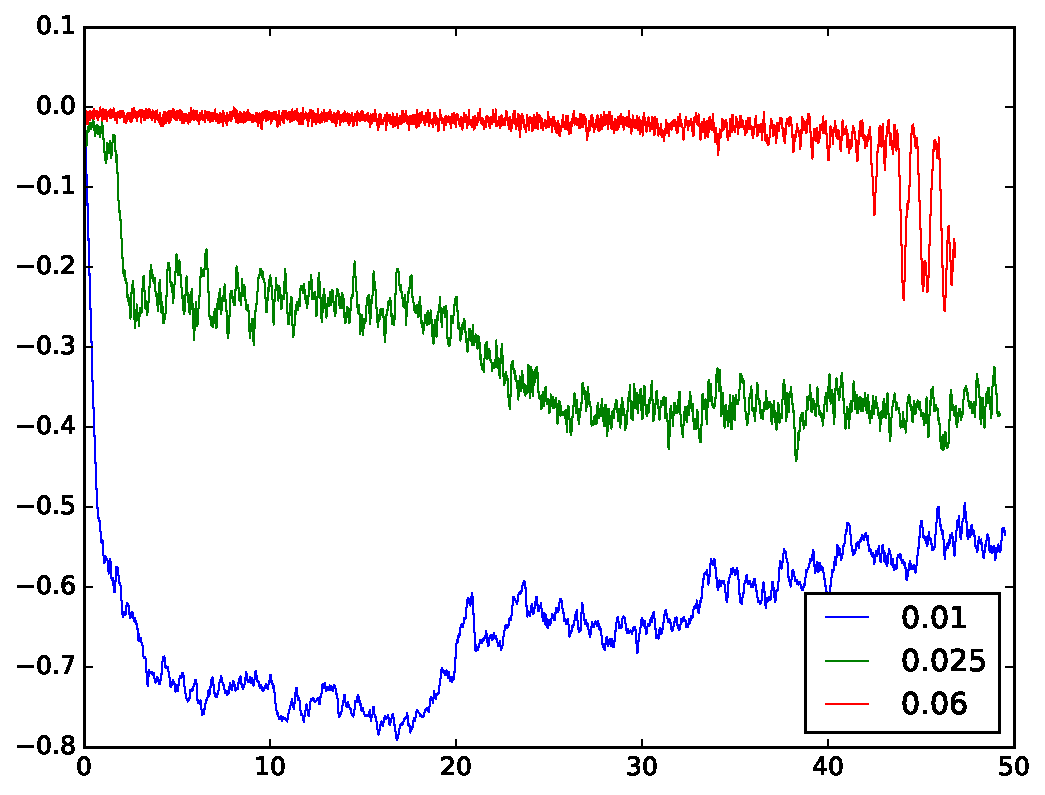
\includegraphics[width=\textwidth]{images/rec_std_ent_reg.pdf}
	\centering
	\caption{Logarithm of average standard deviation of the policy of agents in Figure~\ref{rec_ent_reg}, the horizontal axis is the number of million timesteps.}\label{rec_std_ent_reg}
\end{figure}

\subsection{Experiment on exceptional advantage regularization}
We discuss the effectiveness of exceptional advantage regularization method on multi-modality tasks in this section.

We first demonstrate the general patterns of the distribution on the advantage values on the simple multi-modality task "moveg2". In this task, the goal direction is sampled from 2 opposite directions. The task is much more simple than the "movecont" task because the agent only needs to learn from the image whether it needs to go forward or backward. 

The performance on the total return of an ACKTR agent is shown in Figure~\ref{rec_stat_moveg2}. The performance in terms of average reward per time-step is shown in Figure~\ref{rec_stat_moveg2_meanrt}, and the average standard deviation is shown in Figre~\ref{rec_stat_moveg2_std}.


\begin{figure}[!htbp]
	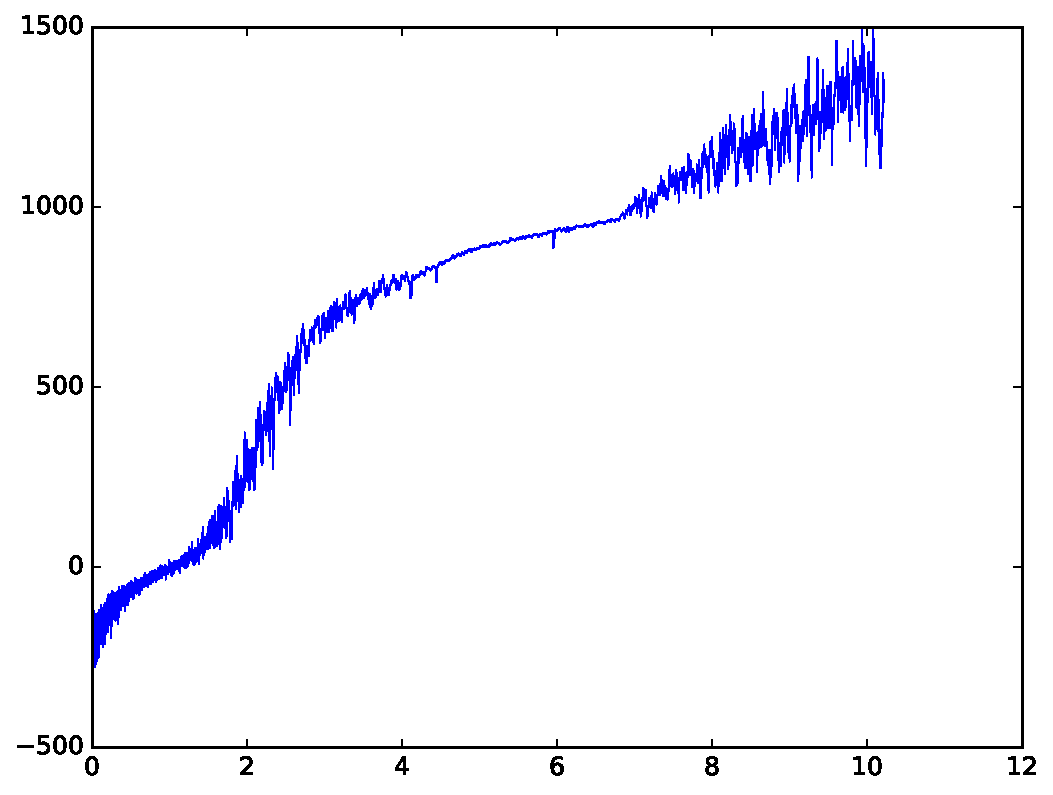
\includegraphics[width=0.7\textwidth]{images/rec_stat_moveg2.pdf}
	\centering
	\caption{Performance of ACKTR agent on the "moveg2" task, the horizontal axis is the number of million timesteps and the vertical axis is the total episode reward averaged over the last 20 episodes}\label{rec_stat_moveg2}
\end{figure}

\begin{figure}[!htbp]
	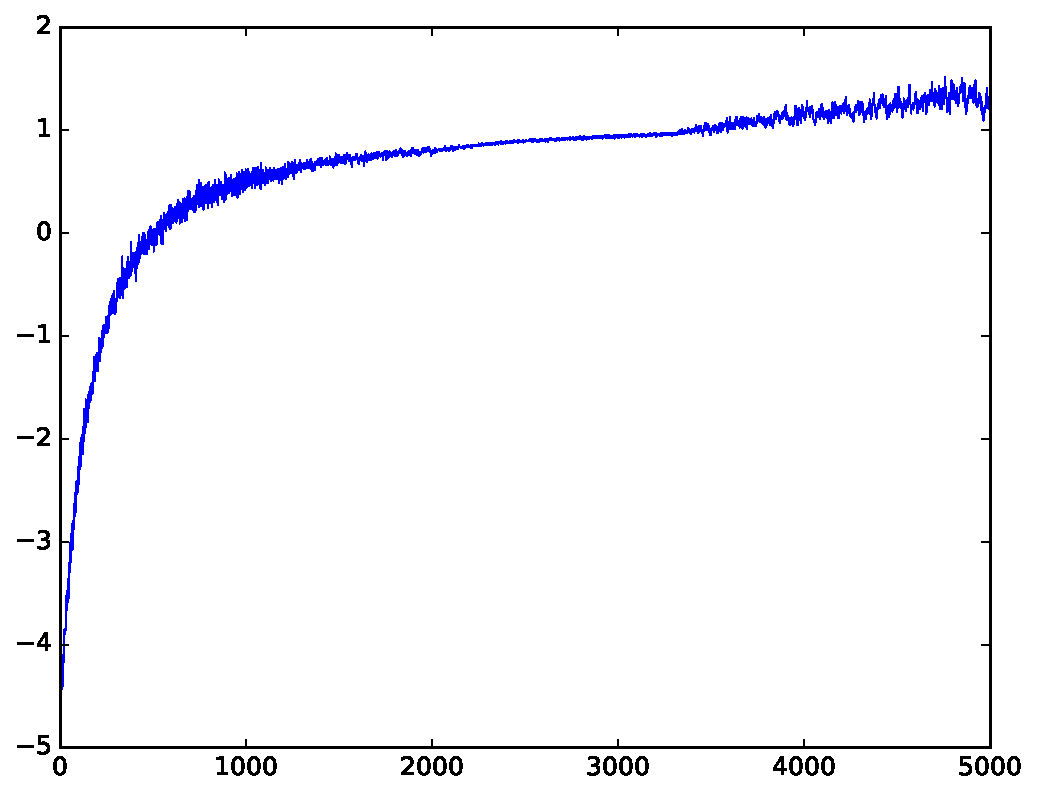
\includegraphics[width=0.7\textwidth]{images/rec_stat_moveg2_meanrt.pdf}
	\centering
	\caption{The avearge reward per time-step of ACKTR agent on the "moveg2" task, the horizontal axis is the number of training batches}\label{rec_stat_moveg2_meanrt}
\end{figure}

\begin{figure}[!htbp]
	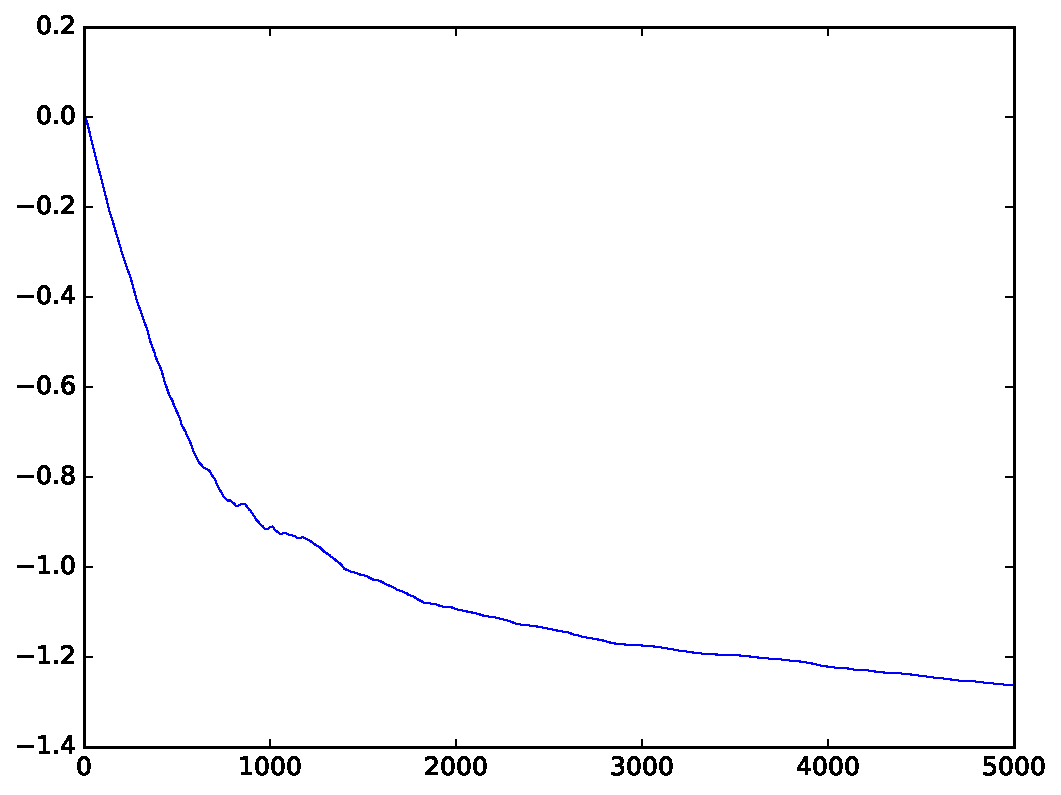
\includegraphics[width=0.7\textwidth]{images/rec_stat_moveg2_std.pdf}
	\centering
	\caption{The logarithm of avearge standard deviation of ACKTR agent's policy on the "moveg2" task, the horizontal axis is the number of training batches}\label{rec_stat_moveg2_std}
\end{figure}
The distribution of advantage values at the first batch (batch 0) is shown in Figure~\ref{vis_stats_0}. It can be seen that the advantage values are distributed uniformly across different values of log-likelihood because the critic model has not been trained. After the critic model has been trained for a reasonable amount of time, the marginal distribution advantage value tend to follow a normal distribution with zero mean. An example is shown in Figure~\ref{vis_stats_3000}, which is the distribution at batch 3000. However, the advantage values are likely to have higher values at low log-likelihood samples when the agent has just escaped from a local minimum. An example is Figure~\ref{vis_stats_4900}, which shows the the distribution of advantage values at batch 4900. It can be seen that the distribution becomes significantly different because many positive advantage points are spread across different log-likelihoods. 

Intuitively, a large number of points with low log-likelihood but high advantage value indicates that the agent needs to increase the degree of exploration. However, the figure~\ref{rec_stat_moveg2_std} on the change of standard deviation shows that the agent actually still keep decreasing the standard deviations of its policy even at this state. Therefore, the application of a exceptional advantage regularization term, could be useful in encouraging exploration in these cases.

\begin{figure}[!htbp]
	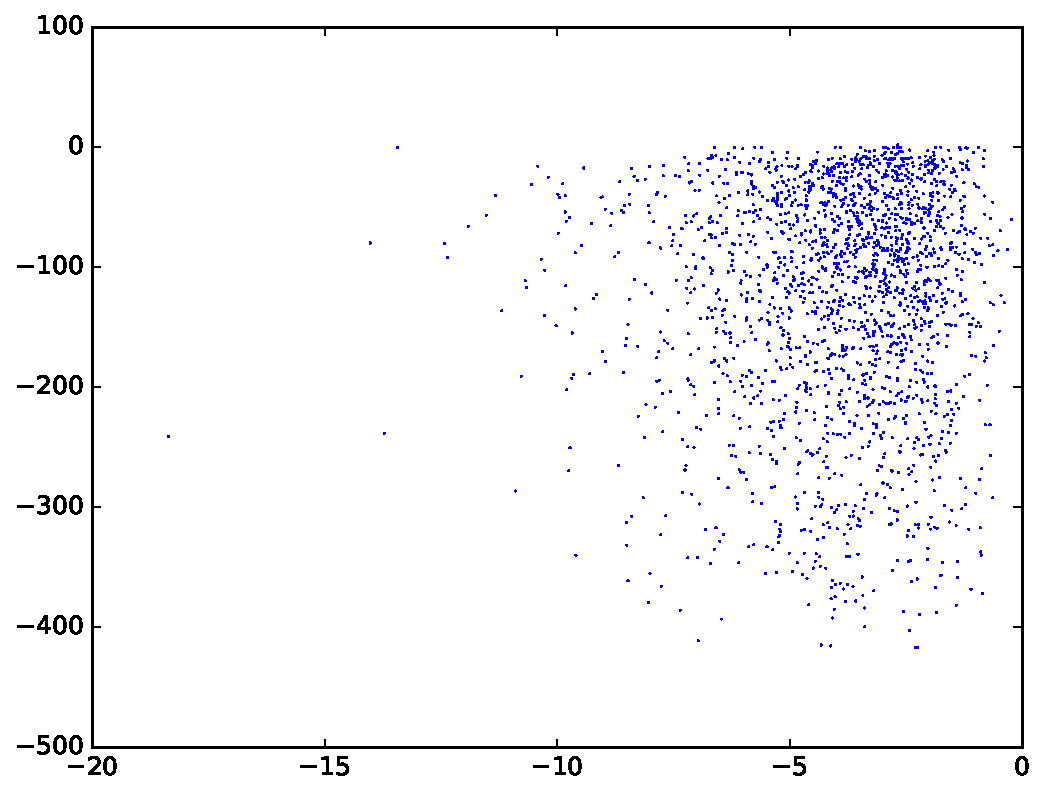
\includegraphics[width=\textwidth]{images/vis_stats_0.pdf}
	\centering
	\caption{The distribution of advantage values of the ACKTR agent at batch 0 on the "moveg2" task, the horizontal axis is the log-likelihood value}
	\label{vis_stats_0}
\end{figure}

\begin{figure}[!htbp]
	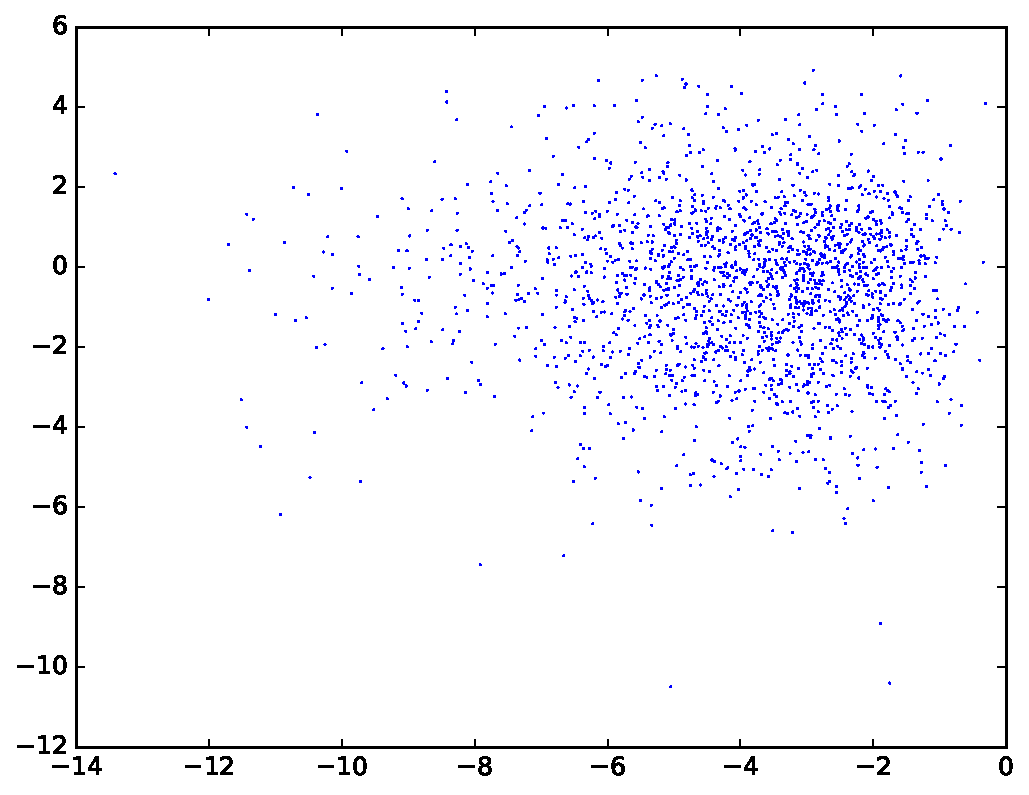
\includegraphics[width=\textwidth]{images/vis_stats_3000.pdf}
	\centering
	\caption{The distribution of advantage values of the ACKTR agent at batch 300 on the "moveg2" task, the horizontal axis is the log-likelihood value}
	\label{vis_stats_3000}
\end{figure}

\begin{figure}[!htbp]
	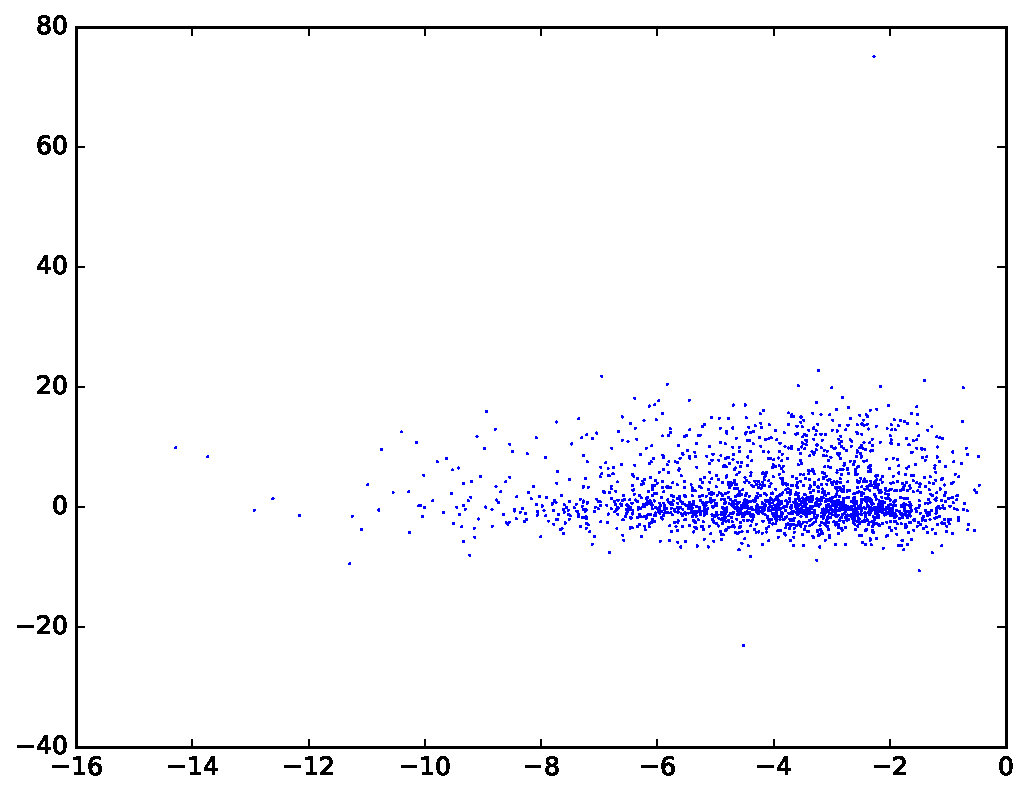
\includegraphics[width=\textwidth]{images/vis_stats_4900.pdf}
	\centering
	\caption{The distribution of advantage values of the ACKTR agent at batch 4900 on the "moveg2" task, the horizontal axis is the log-likelihood value}
	\label{vis_stats_4900}
\end{figure}

We then verify the performance of exceptional advantage regularization on the 'movecont' task.
The performance of an ACKTR agent with different weights exceptional advantage regularization on the in Figure~\ref{rec_adv_reg}, and the average standard deviation parameter of their policies are shown in Figure~\ref{rec_std_adv_reg}. All the agents are trained with batch-size 2560 and KL-divergence constraint 0.0003. The weight-0 agent is the same as the original ACKTR agent without any exploration regularization, and it could only achieve a total reward of around 2000 at the end of training. The agent with exceptional advantage regularization weight 0.04 can improve rapidly in the early phase before 40 million timestep, but gets stuck at around 3500. This shows that the exceptional advantage regularization method could have adverse effect on the convergence of policy in the late phase of training, which is also indicated in by average std curve. The agent with exceptional advantage regularization weight 0.01 achieves the best final performance. Its average standard deviation shows that the agent manages to increase its policy entropy and re-explore the environment after it has escaped from a local minimum.
\begin{figure}[!htbp]
	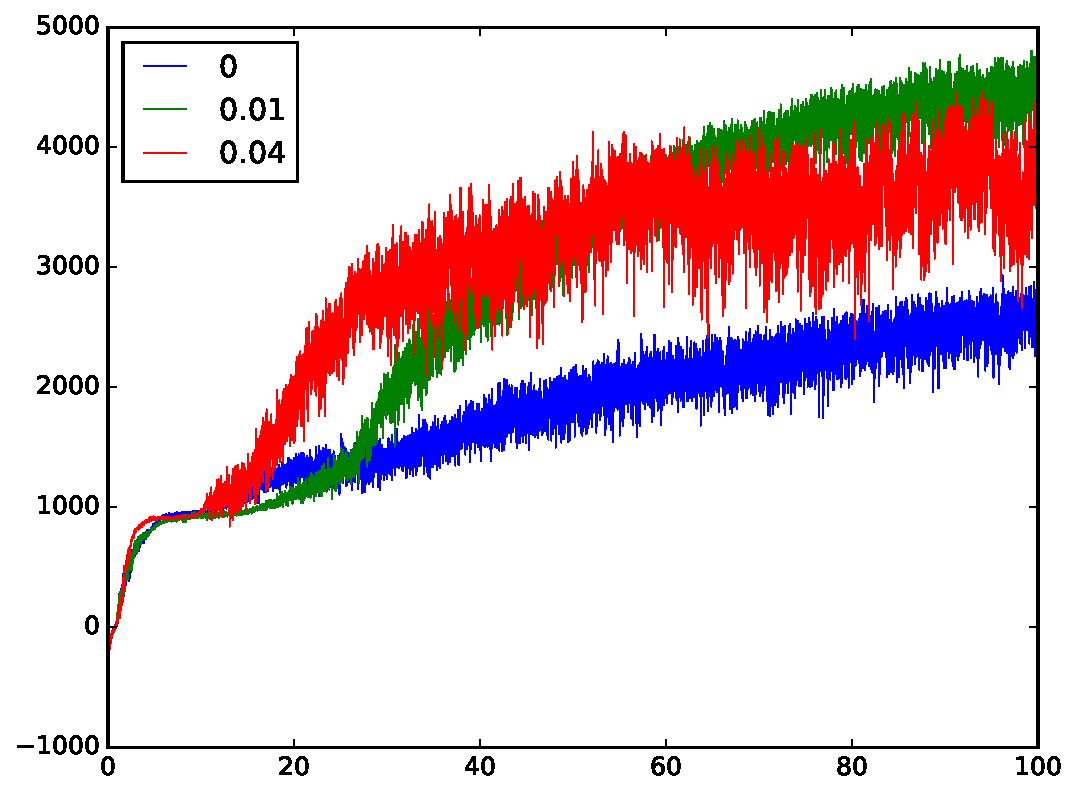
\includegraphics[width=\textwidth]{images/rec_adv_reg.pdf}
	\centering
	\caption{Performance of agents with different exceptional advantage regularization weights, the x-axis is the number of million time-steps and the y-axis is the total episode reward averaged over the last 32 episodes}\label{rec_adv_reg}
\end{figure}

\begin{figure}[!htbp]
	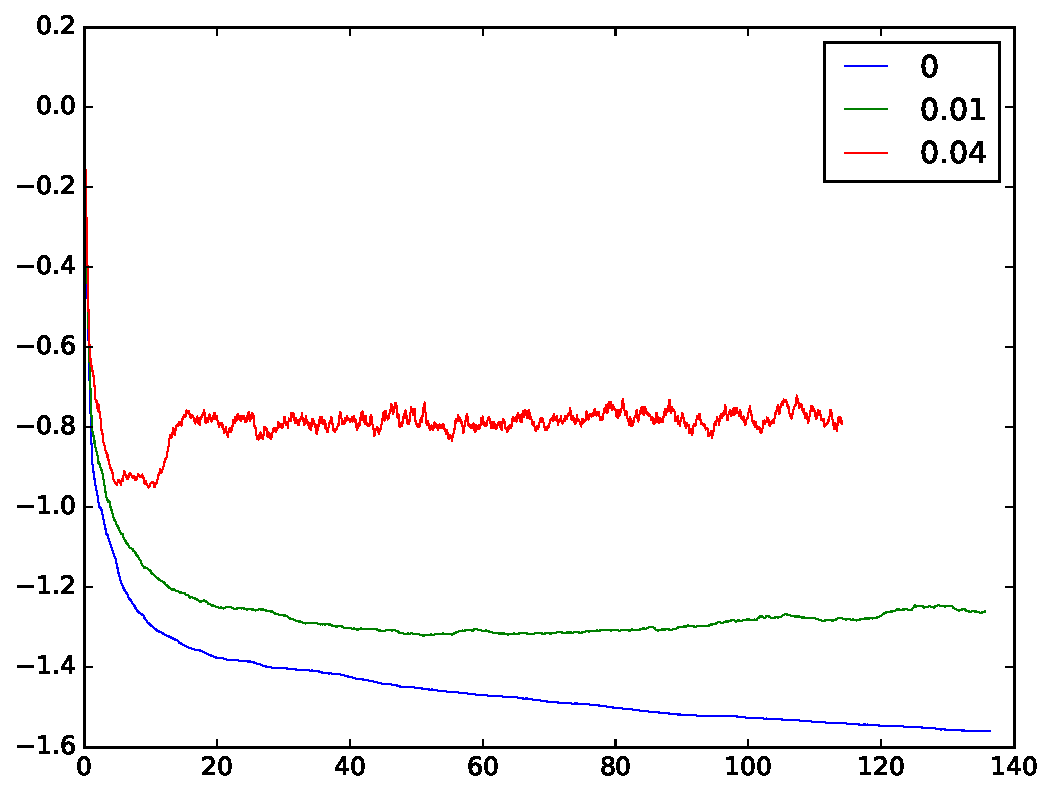
\includegraphics[width=\textwidth]{images/rec_std_adv_reg.pdf}
	\centering
	\caption{The logarithm of avearge standard deviation of agents with different exceptional advantage regularization weights, the horizontal axis is the number of million time-steps and the vertical axis is the total episode reward averaged over the last 32 episodes}\label{rec_std_adv_reg}
\end{figure}

\subsection{Experiment on the Robust Concentric Mixture Gaussian Policy}
The effectiveness of robust concentric mixture Gaussian policy agent in exploration of task "movecont" is verified in this section. 

The performance of an ACKTR mixture Gaussian policy agent is shown in Figure~\ref{rec_mix}. The results shows that the mixture Gaussian policy agents have slower learning rates compared to pure Gaussian policy agents. However, the agents are able to achieve a good fubak performance, with a total reward of around 4000 when the KL-divergence is set properly.

\begin{figure}[!htbp]
	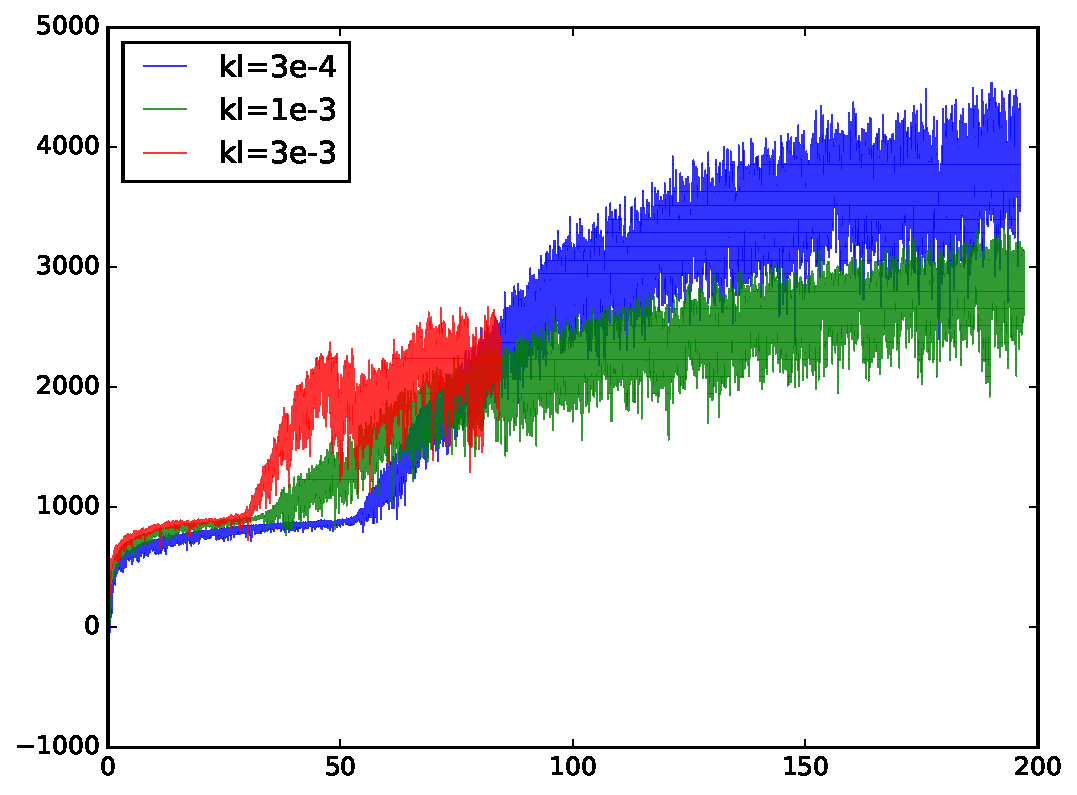
\includegraphics[width=\textwidth]{images/rec_mix.pdf}
	\centering
	\caption{Performance of ACKTR agents with different KL-divergence constraints, the x-axis is the number of million time-steps and the y-axis is the total episode reward averaged over the last 32 episodes}\label{rec_mix}
\end{figure}

% \section{Preliminary experiment on the hierarchical agent architecture}
% A preliminary experiment has been done on training the proposed agent in the dynamic2d environment. The termination policy sets $b_i = 4.5$ and isn't trained during policy updates. The figure is shown in Figure \ref{rec_180419_fix_ter}.

% The result shows that the learning of the root-level policy is effective.


% \begin{figure}[h]
% 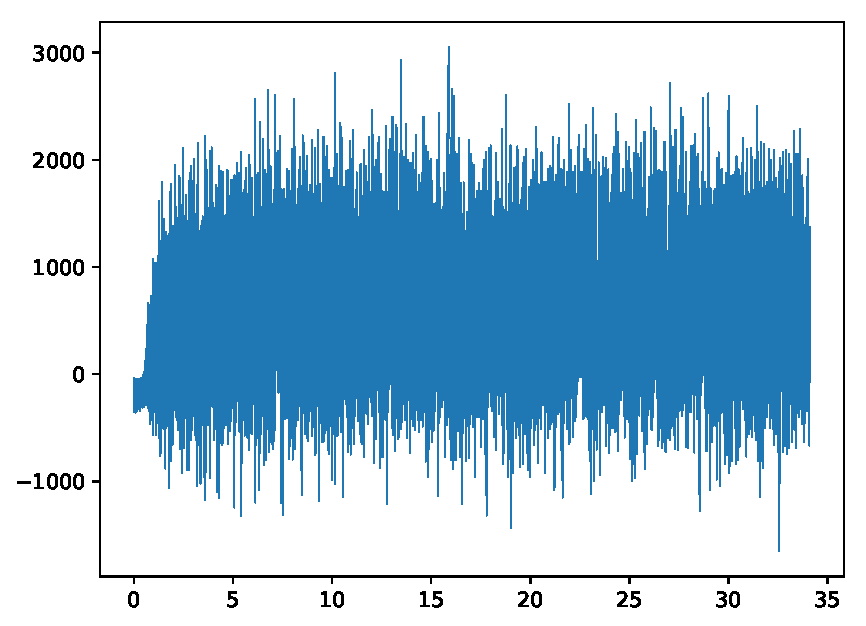
\includegraphics[width=\textwidth]{images/rec_180420_fix_ter.pdf}
% \centering
% \caption{Experiment on dynamic2d on a hierarchical reinforcement learning agent with fixed-length termination policy}
% \end{figure}\label{rec_180419_fix_ter}

% The current guess on the source of stability is that the sub-policy doesn't perform well in the target environment. Figure \ref{rec_180419_fix_ter_len} shows the average episode length of the hierachical agent.

% \begin{figure}[h]
% 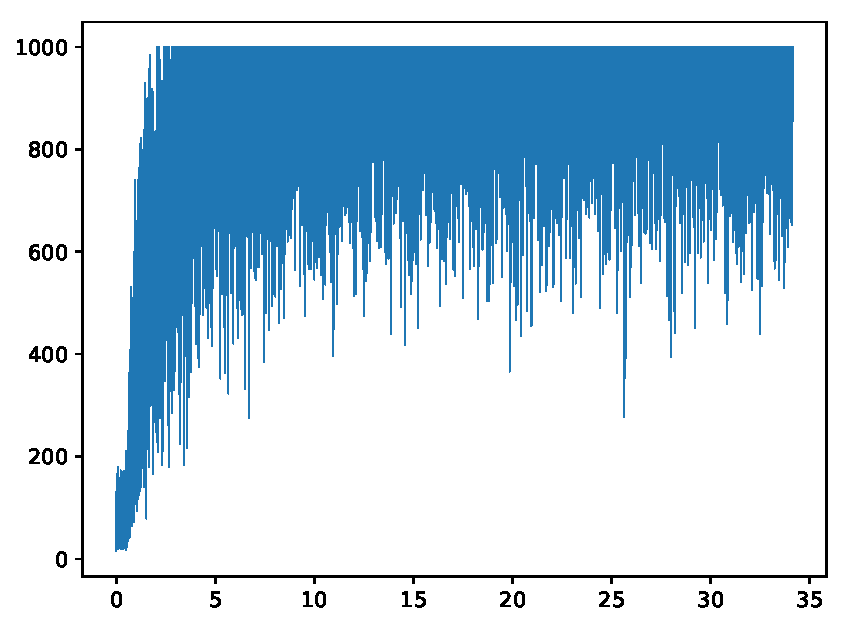
\includegraphics[width=\textwidth]{images/rec_180420_fix_ter_len.pdf}
% \centering
% \caption{The average episode length of the dynamic2d hierarchical agent}
% \end{figure}\label{rec_180419_fix_ter_len}

% \section{Experiment up to April. 26: on transfer of source policies}
% The results show that the source task policy cannot perform well in dynamic2d, because of different initial condition caused by the switching of moving direction.

% An experiment is developed to fine-tune the source task policies during the learning of the target task. However, the problem is on how to fine-tune a Gaussian policy that has already converged with low STD.

% \section{Ongoing development in transfer of actuator policy}
% \section{On training source tasks}
% I found that using a 1-step proximate policy gradient algorithm with an adaptive KL penalty is the most economic method.

% Previously, the ACKTR agent sometimes stuck at a performance around 3000 as discussed in the group meeting in March. The reason could be due to KL divergence constraint is too small. A small change in the mean vector could lead to a large KL divergence when the STD converges to nearly zero. That prevents the agent's policy from improving.

% It is likely that an alternative metric could be better for trust region methods, like L1-error or JS-divergence.
% \subsection{Training the actuator policy from scratch in the target task}
% An experiment is being run to test if the agent can effectively learn the actuator policies. The actuator agent learns stably. However the rate of improvement is slow due to the simultaneous training of all the source tasks. The current per step mean reward reaches 1.5 after 3 days.
% \subsection{Fine-tuning the actuator policies}
% The fine-tuning of the actuator polices seems to fail in the target problem. The performance usually drops during the fine-tuning period. 
% Deeper investigations are undergoing to fix the problem.
% \subsection{Training a transition policy}
% The development of the transition policy is still undergoing.
% \section{On the hierarchical reinforcement learning}
% I found that the current scheduler agent model is unstable in training. 

% I'm trying to develop a mixed type policy network, where the output is a binary variable and the discrete/continuous distribution. The binary variable indicates whether the current actuator policy should be terminated, and the latter one denotes the policy distribution. The relevant properties such as KL divergence for this kind of distribution should be derived and developed.

% \section{Progress by May. 10}
% Current work still focuses on the investigation of transferring actuator policies.
% The current model fails to reproduce the previous positive experiments on multi-modality tasks. I've done several bug-fixes and parameter tuning, however the problem still remains. The cause is still under investigation, one possible cause is related to the stability of actuator policies in terms of failure rate. If an actuator policy is prune to "game over" behaviour when initialized after another actuator policy, the decider agent may tend to constantly choose a fixed policy. 

% \section{Progress by Mar. 17}
% \subsection{Reproduction of the multi-modality environment performance}
% I've just finished fixing the code, so that the new model achieves a reasonable performance in move1d. The performance is shown in Figure \ref{rec_move1d}.
% \begin{figure}[h]
% 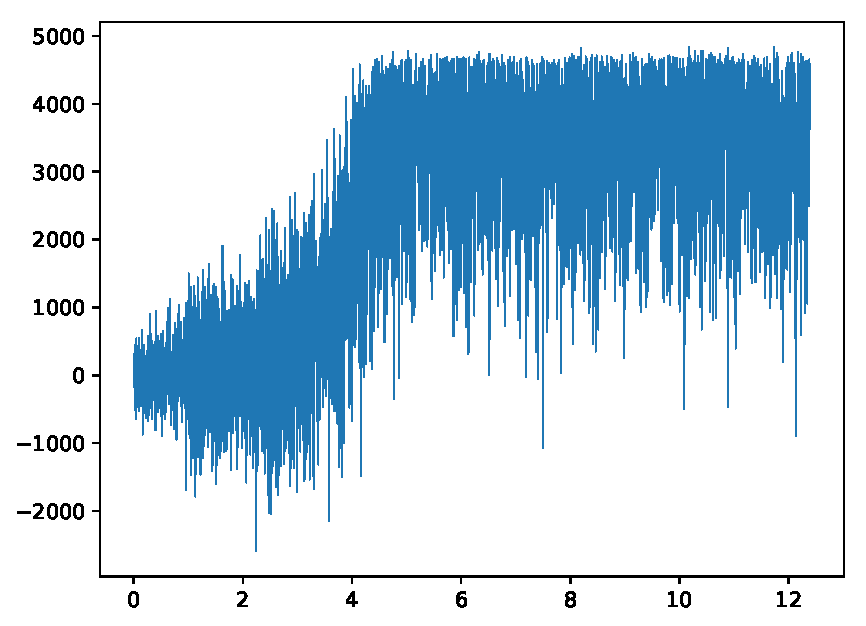
\includegraphics[width=\textwidth]{images/rec_180517_move1d_better.pdf}
% \centering
% \caption{Experiment on move1d}
% \end{figure}\label{rec_move1d}

% \subsection{Study of generalized advantage estimation}
% During the development of the hierarchical reinforcement learning model, I developed a modified version of \cite{schulman2015high} for hierarchical reinforcement learning methods. I found a problem that the original method didn't correctly normalize the advantage values $A_t$ according to $\sum_{i=t}^{i=t+T}\lambda^{i}$. That would lead to a advantage values linearly increasing magnitudes with the increased time to termination. However, I found that the correct method doesn't produce a better result according to the experiments up to now.

% \subsection{Policy gradient methods with Wasserstein metric}
% I found that one problem with the current KL-divergence based trust region methods is that agents will find it difficult to learn after the STD of the Gaussian policy approaches zero, due to the sensitive KL-divergence loss. I found that it seems better to replace the KL-divergence metric with Wasserstein metric for Gaussian policies.

% A preliminary experiment is done on the original Ant task and has shown positive results, which is shown in Figure \ref{rec_wass}. The proposed agent is the policy gradient agent with adaptive Wasserstein metric penalty.

% \begin{figure}[h]
% 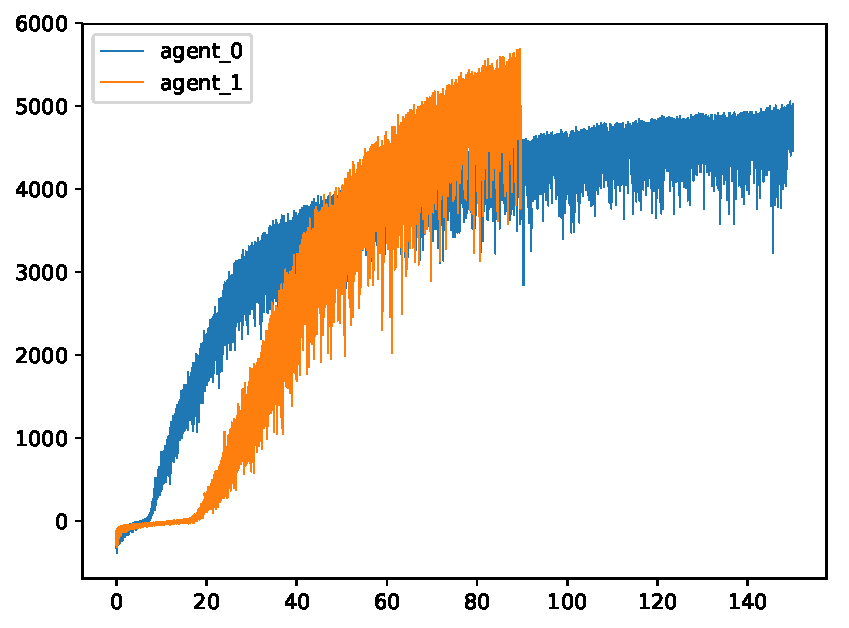
\includegraphics[width=\textwidth]{images/rec_180517_wasserstein.pdf}
% \centering
% \caption{Experiment comparison on Wasserstein metric and KL divergence. agent\_1 is the Wasserstein agent}

% \end{figure}\label{rec_wass}


%!TEX program = xelatex
%!TEX root = ./thesis.tex
\chapter{Discussion}
This thesis studies reinforcement learning solutions to robot control tasks with multi-modal state space and sparse reward functions.

Firstly, we have proposed a set of experiment environments and shown that contemporary deep reinforcement learning algorithms for continuous control are not good at solving them. 

Secondly, we have proposed several techniques aiming to improve the performance of the contemporary flat reinforcement learning methods, including Wasserstein actor critic Kronecker-factored trust region policy optimization (W-KTR) method, exceptional advantage estimation, and robust concentric Gaussian mixture model. Some of them, especially the exceptional advantage estimation method, lead to improvement on the final performance of the agent. However, an efficient flat reinforcement learning solution to multi-modal state-space problems is still missing. It is worth exploring in the future whether there could be any method that could completely solve the local minimum problem of multi-modal state-space problems.

Thirdly, we have proposed the flexible-scheduling hierarchical method for the tasks with multi-modal state space and sparse reward functions given a predefined set of source tasks. The experiments show positive results in that the proposed method can learn to solve the tasks in an end-to-end manner.

The experiments in this thesis only show preliminary results on a limited set of tasks. The capability of the method on general robot problems also needs to be verified on a bigger variety of problems in future works. The drawback of this hierarchical reinforcement learning framework is that it requires a properly pre-defined set of source tasks. Designing the source-task set is easy for the proposed problems, but we are not sure whether the job is feasible for realistic tasks in general. Apart from that, we have not thoroughly investigated how the scheduling of the decision policy training and switcher policy training could be designed. We have a pre-defined switcher policy at first, and schedule the training of decision policy and switcher policy into two separate phases in our experiments. Future works can investigate whether it is possible to train the decision policy and the switcher policy jointly. Apart from that, how to properly balance the switcher policy for better reinforcement learning performance and lower decision frequency of the decider policy is worth studying.

In conclusion, realistic continuous control tasks with multi-modal state space and sparse reward functions still pose a significant challenge to flat and hierarchical reinforcement learning methods. Our study proposes several novel solutions, but an efficient solution that achieves optimal performance without human intervention is still missing.
%!TEX program = xelatex
%!TEX root = ./thesis.tex
% \chapter{another}

\newpage
\addcontentsline{toc}{chapter}{Reference}
\bibliographystyle{IEEEtran}
%\bibliographystyle{IEEEtran}
\bibliography{reference} 

\newpage
\addcontentsline{toc}{chapter}{Publication}
% \null\skip0.2in
% \begin{center}
% {\bf \Large \underline{List of Publications}}
% \end{center}
% \vspace{12mm}


% 1. Publication 1

% 2. Publicstion 2


\newpage
\addcontentsline{toc}{chapter}{Appendix}
\appendix
%!TEX program = xelatex
%!TEX root = ./thesis.tex
\chapter{Appendix 1}


\end{document}
